% Options for packages loaded elsewhere
\PassOptionsToPackage{unicode}{hyperref}
\PassOptionsToPackage{hyphens}{url}
%
\documentclass[
  12pt,
]{article}
\title{Precipitation Change in Beaufort}
\usepackage{etoolbox}
\makeatletter
\providecommand{\subtitle}[1]{% add subtitle to \maketitle
  \apptocmd{\@title}{\par {\large #1 \par}}{}{}
}
\makeatother
\subtitle{Web address for GitHub repository}
\author{Karen Thornton, Lambert Ngenzi, Taro Katayama}
\date{}

\usepackage{amsmath,amssymb}
\usepackage{lmodern}
\usepackage{iftex}
\ifPDFTeX
  \usepackage[T1]{fontenc}
  \usepackage[utf8]{inputenc}
  \usepackage{textcomp} % provide euro and other symbols
\else % if luatex or xetex
  \usepackage{unicode-math}
  \defaultfontfeatures{Scale=MatchLowercase}
  \defaultfontfeatures[\rmfamily]{Ligatures=TeX,Scale=1}
  \setmainfont[]{Times New Roman}
\fi
% Use upquote if available, for straight quotes in verbatim environments
\IfFileExists{upquote.sty}{\usepackage{upquote}}{}
\IfFileExists{microtype.sty}{% use microtype if available
  \usepackage[]{microtype}
  \UseMicrotypeSet[protrusion]{basicmath} % disable protrusion for tt fonts
}{}
\makeatletter
\@ifundefined{KOMAClassName}{% if non-KOMA class
  \IfFileExists{parskip.sty}{%
    \usepackage{parskip}
  }{% else
    \setlength{\parindent}{0pt}
    \setlength{\parskip}{6pt plus 2pt minus 1pt}}
}{% if KOMA class
  \KOMAoptions{parskip=half}}
\makeatother
\usepackage{xcolor}
\IfFileExists{xurl.sty}{\usepackage{xurl}}{} % add URL line breaks if available
\IfFileExists{bookmark.sty}{\usepackage{bookmark}}{\usepackage{hyperref}}
\hypersetup{
  pdftitle={Precipitation Change in Beaufort},
  pdfauthor={Karen Thornton, Lambert Ngenzi, Taro Katayama},
  hidelinks,
  pdfcreator={LaTeX via pandoc}}
\urlstyle{same} % disable monospaced font for URLs
\usepackage[margin=2.54cm]{geometry}
\usepackage{color}
\usepackage{fancyvrb}
\newcommand{\VerbBar}{|}
\newcommand{\VERB}{\Verb[commandchars=\\\{\}]}
\DefineVerbatimEnvironment{Highlighting}{Verbatim}{commandchars=\\\{\}}
% Add ',fontsize=\small' for more characters per line
\usepackage{framed}
\definecolor{shadecolor}{RGB}{248,248,248}
\newenvironment{Shaded}{\begin{snugshade}}{\end{snugshade}}
\newcommand{\AlertTok}[1]{\textcolor[rgb]{0.94,0.16,0.16}{#1}}
\newcommand{\AnnotationTok}[1]{\textcolor[rgb]{0.56,0.35,0.01}{\textbf{\textit{#1}}}}
\newcommand{\AttributeTok}[1]{\textcolor[rgb]{0.77,0.63,0.00}{#1}}
\newcommand{\BaseNTok}[1]{\textcolor[rgb]{0.00,0.00,0.81}{#1}}
\newcommand{\BuiltInTok}[1]{#1}
\newcommand{\CharTok}[1]{\textcolor[rgb]{0.31,0.60,0.02}{#1}}
\newcommand{\CommentTok}[1]{\textcolor[rgb]{0.56,0.35,0.01}{\textit{#1}}}
\newcommand{\CommentVarTok}[1]{\textcolor[rgb]{0.56,0.35,0.01}{\textbf{\textit{#1}}}}
\newcommand{\ConstantTok}[1]{\textcolor[rgb]{0.00,0.00,0.00}{#1}}
\newcommand{\ControlFlowTok}[1]{\textcolor[rgb]{0.13,0.29,0.53}{\textbf{#1}}}
\newcommand{\DataTypeTok}[1]{\textcolor[rgb]{0.13,0.29,0.53}{#1}}
\newcommand{\DecValTok}[1]{\textcolor[rgb]{0.00,0.00,0.81}{#1}}
\newcommand{\DocumentationTok}[1]{\textcolor[rgb]{0.56,0.35,0.01}{\textbf{\textit{#1}}}}
\newcommand{\ErrorTok}[1]{\textcolor[rgb]{0.64,0.00,0.00}{\textbf{#1}}}
\newcommand{\ExtensionTok}[1]{#1}
\newcommand{\FloatTok}[1]{\textcolor[rgb]{0.00,0.00,0.81}{#1}}
\newcommand{\FunctionTok}[1]{\textcolor[rgb]{0.00,0.00,0.00}{#1}}
\newcommand{\ImportTok}[1]{#1}
\newcommand{\InformationTok}[1]{\textcolor[rgb]{0.56,0.35,0.01}{\textbf{\textit{#1}}}}
\newcommand{\KeywordTok}[1]{\textcolor[rgb]{0.13,0.29,0.53}{\textbf{#1}}}
\newcommand{\NormalTok}[1]{#1}
\newcommand{\OperatorTok}[1]{\textcolor[rgb]{0.81,0.36,0.00}{\textbf{#1}}}
\newcommand{\OtherTok}[1]{\textcolor[rgb]{0.56,0.35,0.01}{#1}}
\newcommand{\PreprocessorTok}[1]{\textcolor[rgb]{0.56,0.35,0.01}{\textit{#1}}}
\newcommand{\RegionMarkerTok}[1]{#1}
\newcommand{\SpecialCharTok}[1]{\textcolor[rgb]{0.00,0.00,0.00}{#1}}
\newcommand{\SpecialStringTok}[1]{\textcolor[rgb]{0.31,0.60,0.02}{#1}}
\newcommand{\StringTok}[1]{\textcolor[rgb]{0.31,0.60,0.02}{#1}}
\newcommand{\VariableTok}[1]{\textcolor[rgb]{0.00,0.00,0.00}{#1}}
\newcommand{\VerbatimStringTok}[1]{\textcolor[rgb]{0.31,0.60,0.02}{#1}}
\newcommand{\WarningTok}[1]{\textcolor[rgb]{0.56,0.35,0.01}{\textbf{\textit{#1}}}}
\usepackage{longtable,booktabs,array}
\usepackage{calc} % for calculating minipage widths
% Correct order of tables after \paragraph or \subparagraph
\usepackage{etoolbox}
\makeatletter
\patchcmd\longtable{\par}{\if@noskipsec\mbox{}\fi\par}{}{}
\makeatother
% Allow footnotes in longtable head/foot
\IfFileExists{footnotehyper.sty}{\usepackage{footnotehyper}}{\usepackage{footnote}}
\makesavenoteenv{longtable}
\usepackage{graphicx}
\makeatletter
\def\maxwidth{\ifdim\Gin@nat@width>\linewidth\linewidth\else\Gin@nat@width\fi}
\def\maxheight{\ifdim\Gin@nat@height>\textheight\textheight\else\Gin@nat@height\fi}
\makeatother
% Scale images if necessary, so that they will not overflow the page
% margins by default, and it is still possible to overwrite the defaults
% using explicit options in \includegraphics[width, height, ...]{}
\setkeys{Gin}{width=\maxwidth,height=\maxheight,keepaspectratio}
% Set default figure placement to htbp
\makeatletter
\def\fps@figure{htbp}
\makeatother
\setlength{\emergencystretch}{3em} % prevent overfull lines
\providecommand{\tightlist}{%
  \setlength{\itemsep}{0pt}\setlength{\parskip}{0pt}}
\setcounter{secnumdepth}{5}
\ifLuaTeX
  \usepackage{selnolig}  % disable illegal ligatures
\fi

\begin{document}
\maketitle

\newpage
\tableofcontents 
\newpage
\listoftables 
\newpage
\listoffigures 
\newpage

Initial steps * get data * Wrangle data * graph data to see what we're
working with * try a seasonal Mann-kendall test * divide decades and see
if there's a statistical significant difference * Optional: map of three
schools in NC * Make presentation

Wrangle Data

\begin{Shaded}
\begin{Highlighting}[]
\CommentTok{\#Created monthly mean precipitation + total monthly precipitation dataset for Beaufort. This dataset only for visualization purposes}
\NormalTok{Beaufort\_Clean}\OtherTok{\textless{}{-}}\NormalTok{ Beaufort\_RAW}\SpecialCharTok{\%\textgreater{}\%}
  \FunctionTok{group\_by}\NormalTok{(year,month)}\SpecialCharTok{\%\textgreater{}\%}
   \FunctionTok{summarise}\NormalTok{(}\AttributeTok{meanmonthlyprecip=} \FunctionTok{mean}\NormalTok{(Mean\_Precip\_mm),}
             \AttributeTok{sumMonthlyPrecip=} \FunctionTok{sum}\NormalTok{(Mean\_Precip\_mm))}\SpecialCharTok{\%\textgreater{}\%}
  \FunctionTok{mutate}\NormalTok{(}\AttributeTok{Date=} \FunctionTok{my}\NormalTok{(}\FunctionTok{paste0}\NormalTok{(month,}\StringTok{"{-}"}\NormalTok{, year)))}
\end{Highlighting}
\end{Shaded}

\begin{verbatim}
## `summarise()` has grouped output by 'year'. You can override using the `.groups` argument.
\end{verbatim}

\begin{Shaded}
\begin{Highlighting}[]
\CommentTok{\#10 year time frame, precipitation in inches (1997{-}01{-}01 to 2006{-}12{-}31) +significant 24hr precipitation events in magnitude+ \# of significant precipitation events}
\NormalTok{Beaufort\_early}\OtherTok{\textless{}{-}}\NormalTok{ Beaufort\_RAW}\SpecialCharTok{\%\textgreater{}\%}
  \FunctionTok{mutate}\NormalTok{(}\AttributeTok{PrecipInches=}\NormalTok{ Mean\_Precip\_mm}\SpecialCharTok{*}\FloatTok{0.0394}\NormalTok{)}\SpecialCharTok{\%\textgreater{}\%}
  \FunctionTok{filter}\NormalTok{(Date }\SpecialCharTok{\textgreater{}}\NormalTok{(}\StringTok{"1996{-}12{-}31"}\NormalTok{), Date }\SpecialCharTok{\textless{}}\NormalTok{ (}\StringTok{"2007{-}01{-}01"}\NormalTok{)) }\SpecialCharTok{\%\textgreater{}\%} 
  \FunctionTok{mutate}\NormalTok{(}\AttributeTok{sigPrecip=} \FunctionTok{ifelse}\NormalTok{(PrecipInches}\SpecialCharTok{\textgreater{}}\FloatTok{3.66}\NormalTok{,PrecipInches,}\DecValTok{0}\NormalTok{),}
         \AttributeTok{NumSigPrecip=} \FunctionTok{ifelse}\NormalTok{(PrecipInches}\SpecialCharTok{\textgreater{}}\FloatTok{3.66}\NormalTok{, }\DecValTok{1}\NormalTok{,}\DecValTok{0}\NormalTok{))}\SpecialCharTok{\%\textgreater{}\%}
  \FunctionTok{select}\NormalTok{(Date , year, month, }
\NormalTok{         day\_of\_month, PrecipInches, sigPrecip, NumSigPrecip)}\SpecialCharTok{\%\textgreater{}\%}
  \FunctionTok{drop\_na}\NormalTok{()}
  
\CommentTok{\#Created Beaufort early dataset, where non significant precipitation events were classified as NA.}
\NormalTok{Beaufort\_earlyNo0Precip}\OtherTok{\textless{}{-}}\NormalTok{Beaufort\_RAW}\SpecialCharTok{\%\textgreater{}\%}
  \FunctionTok{mutate}\NormalTok{(}\AttributeTok{PrecipInches=}\NormalTok{Mean\_Precip\_mm}\SpecialCharTok{*}\FloatTok{0.0394}\NormalTok{)}\SpecialCharTok{\%\textgreater{}\%}
  \FunctionTok{filter}\NormalTok{(Date }\SpecialCharTok{\textgreater{}}\NormalTok{(}\StringTok{"1996{-}12{-}31"}\NormalTok{), Date }\SpecialCharTok{\textless{}}\NormalTok{ (}\StringTok{"2007{-}01{-}01"}\NormalTok{)) }\SpecialCharTok{\%\textgreater{}\%} 
  \FunctionTok{mutate}\NormalTok{(}\AttributeTok{sigPrecip=} \FunctionTok{ifelse}\NormalTok{(PrecipInches}\SpecialCharTok{\textgreater{}}\FloatTok{3.66}\NormalTok{,PrecipInches,}\ConstantTok{NA}\NormalTok{),}
         \AttributeTok{NumSigPrecip=} \FunctionTok{ifelse}\NormalTok{(PrecipInches}\SpecialCharTok{\textgreater{}}\FloatTok{3.66}\NormalTok{, }\DecValTok{1}\NormalTok{,}\DecValTok{0}\NormalTok{))}\SpecialCharTok{\%\textgreater{}\%}
  \FunctionTok{select}\NormalTok{(Date , year, month, }
\NormalTok{         day\_of\_month, PrecipInches, sigPrecip, NumSigPrecip)}\SpecialCharTok{\%\textgreater{}\%}
  \FunctionTok{drop\_na}\NormalTok{()}

\CommentTok{\#Summary of number of sig events per year}
\NormalTok{Beaufort\_early\_summary}\OtherTok{\textless{}{-}}\NormalTok{ Beaufort\_early}\SpecialCharTok{\%\textgreater{}\%}
  \FunctionTok{group\_by}\NormalTok{(year)}\SpecialCharTok{\%\textgreater{}\%}
  \FunctionTok{summarise}\NormalTok{(}\AttributeTok{SigPrecipEvents=} \FunctionTok{sum}\NormalTok{(NumSigPrecip))}

\CommentTok{\#Created table of number of significant events per year.}
\NormalTok{EarlyTable}\OtherTok{\textless{}{-}} \FunctionTok{kable}\NormalTok{(Beaufort\_early\_summary, }\AttributeTok{caption =} \StringTok{"Significant Events Over Year"}\NormalTok{)}
\NormalTok{EarlyTable}
\end{Highlighting}
\end{Shaded}

\begin{longtable}[]{@{}rr@{}}
\caption{Significant Events Over Year}\tabularnewline
\toprule
year & SigPrecipEvents \\
\midrule
\endfirsthead
\toprule
year & SigPrecipEvents \\
\midrule
\endhead
1997 & 0 \\
1998 & 1 \\
1999 & 1 \\
2000 & 0 \\
2001 & 0 \\
2002 & 0 \\
2003 & 0 \\
2004 & 0 \\
2005 & 1 \\
2006 & 1 \\
\bottomrule
\end{longtable}

\begin{Shaded}
\begin{Highlighting}[]
\CommentTok{\#Created figure with \# and magnitude of significant events per year.}
\FunctionTok{ggplot}\NormalTok{(Beaufort\_earlyNo0Precip, }\FunctionTok{aes}\NormalTok{(}\AttributeTok{x=}\NormalTok{Date , }\AttributeTok{y=}\NormalTok{sigPrecip))}\SpecialCharTok{+}
  \FunctionTok{geom\_point}\NormalTok{()}
\end{Highlighting}
\end{Shaded}

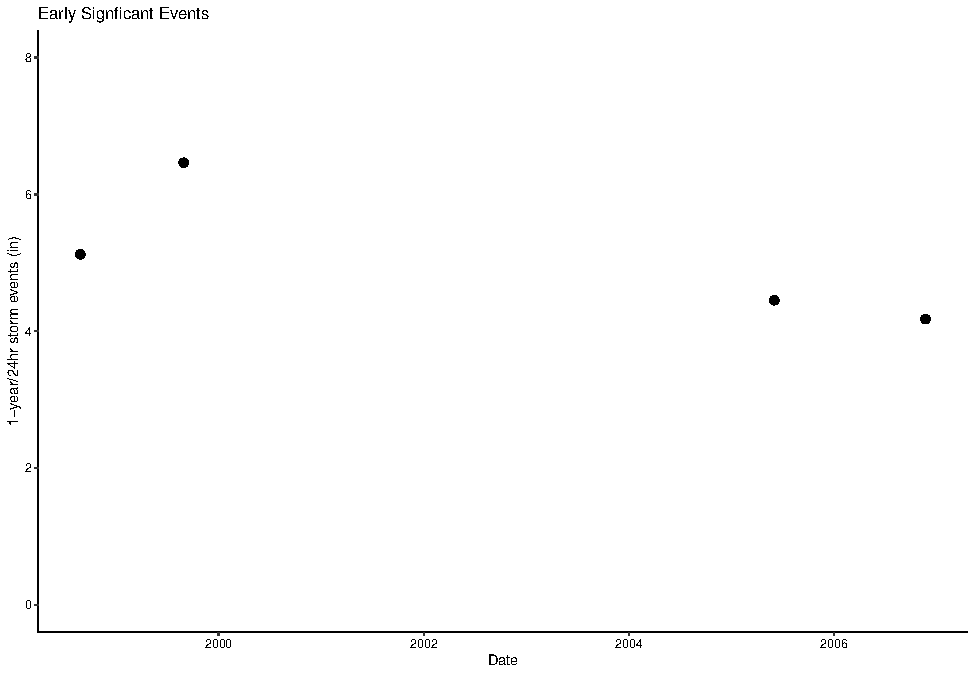
\includegraphics{Project_Template_TLK_files/figure-latex/early-1.pdf}

\begin{Shaded}
\begin{Highlighting}[]
\CommentTok{\#10 year time frame, precipitation in inches (2007{-}01{-}01 to 2016{-}12{-}30) +significant 24hr precipitation events in magnitude + \# of significant precipitation events}
\NormalTok{Beaufort\_Late}\OtherTok{\textless{}{-}}\NormalTok{ Beaufort\_RAW}\SpecialCharTok{\%\textgreater{}\%}
  \FunctionTok{mutate}\NormalTok{(}\AttributeTok{PrecipInches=}\NormalTok{ Mean\_Precip\_mm}\SpecialCharTok{*}\FloatTok{0.0394}\NormalTok{)}\SpecialCharTok{\%\textgreater{}\%}
  \FunctionTok{filter}\NormalTok{(Date }\SpecialCharTok{\textgreater{}} \StringTok{"2006{-}12{-}31"}\NormalTok{)}\SpecialCharTok{\%\textgreater{}\%}
  \FunctionTok{mutate}\NormalTok{(}\AttributeTok{sigPrecip=} \FunctionTok{ifelse}\NormalTok{(PrecipInches}\SpecialCharTok{\textgreater{}}\FloatTok{3.66}\NormalTok{,PrecipInches,}\DecValTok{0}\NormalTok{),}
         \AttributeTok{NumSigPrecip=} \FunctionTok{ifelse}\NormalTok{(PrecipInches}\SpecialCharTok{\textgreater{}}\FloatTok{3.66}\NormalTok{, }\DecValTok{1}\NormalTok{,}\DecValTok{0}\NormalTok{))}\SpecialCharTok{\%\textgreater{}\%}
  \FunctionTok{select}\NormalTok{(Date, year, month, }
\NormalTok{         day\_of\_month, PrecipInches, sigPrecip, NumSigPrecip)}\SpecialCharTok{\%\textgreater{}\%}
  \FunctionTok{drop\_na}\NormalTok{()}

\CommentTok{\#Created Beaufort late dataset, where non significant precipitation events were classified as NA.}
\NormalTok{Beaufort\_LateNo0Precip}\OtherTok{\textless{}{-}}\NormalTok{ Beaufort\_RAW}\SpecialCharTok{\%\textgreater{}\%}
  \FunctionTok{mutate}\NormalTok{(}\AttributeTok{PrecipInches=}\NormalTok{ Mean\_Precip\_mm}\SpecialCharTok{*}\FloatTok{0.0394}\NormalTok{)}\SpecialCharTok{\%\textgreater{}\%}
  \FunctionTok{filter}\NormalTok{(Date }\SpecialCharTok{\textgreater{}} \StringTok{"2006{-}12{-}31"}\NormalTok{)}\SpecialCharTok{\%\textgreater{}\%}
  \FunctionTok{mutate}\NormalTok{(}\AttributeTok{sigPrecip=} \FunctionTok{ifelse}\NormalTok{(PrecipInches}\SpecialCharTok{\textgreater{}}\FloatTok{3.66}\NormalTok{,PrecipInches,}\ConstantTok{NA}\NormalTok{),}
         \AttributeTok{NumSigPrecip=} \FunctionTok{ifelse}\NormalTok{(PrecipInches}\SpecialCharTok{\textgreater{}}\FloatTok{3.66}\NormalTok{, }\DecValTok{1}\NormalTok{,}\DecValTok{0}\NormalTok{))}\SpecialCharTok{\%\textgreater{}\%}
  \FunctionTok{select}\NormalTok{(Date, year, month, }
\NormalTok{         day\_of\_month, PrecipInches, sigPrecip, NumSigPrecip)}\SpecialCharTok{\%\textgreater{}\%}
  \FunctionTok{drop\_na}\NormalTok{()}

\CommentTok{\#Summary of number of sig events per year (Late)}
\NormalTok{Beaufort\_late\_summary}\OtherTok{\textless{}{-}}\NormalTok{ Beaufort\_Late}\SpecialCharTok{\%\textgreater{}\%}
  \FunctionTok{group\_by}\NormalTok{(year)}\SpecialCharTok{\%\textgreater{}\%}
  \FunctionTok{summarise}\NormalTok{(}\AttributeTok{SigPrecipEvents=} \FunctionTok{sum}\NormalTok{(NumSigPrecip))}

\CommentTok{\#Created figure with \# and magnitude of significant events per year.}
\FunctionTok{ggplot}\NormalTok{(Beaufort\_LateNo0Precip, }\FunctionTok{aes}\NormalTok{(}\AttributeTok{x=}\NormalTok{Date , }\AttributeTok{y=}\NormalTok{sigPrecip))}\SpecialCharTok{+}
  \FunctionTok{geom\_point}\NormalTok{()}
\end{Highlighting}
\end{Shaded}

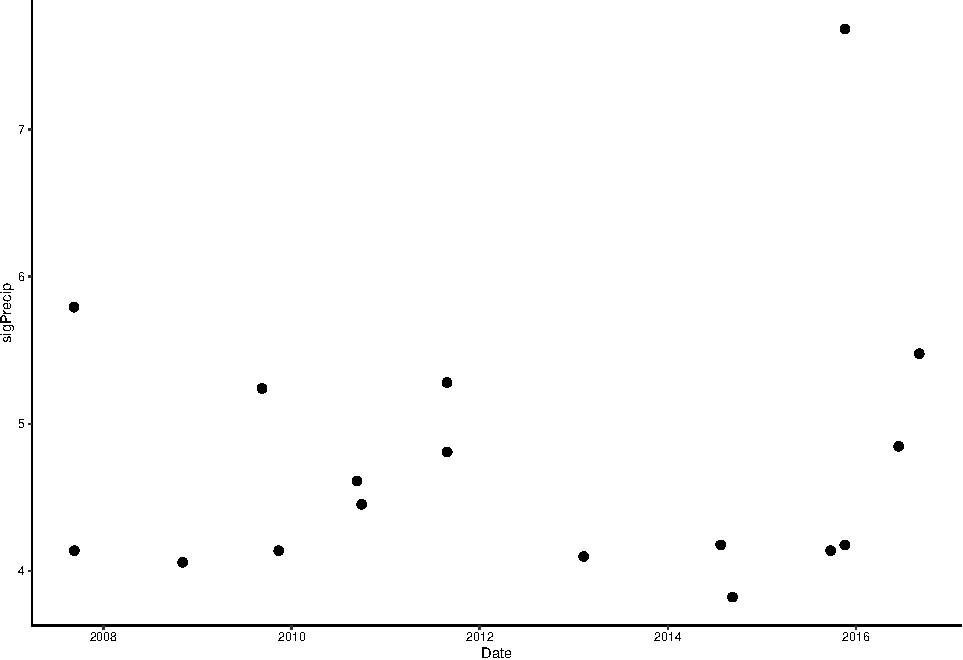
\includegraphics{Project_Template_TLK_files/figure-latex/late-1.pdf}

\begin{Shaded}
\begin{Highlighting}[]
\CommentTok{\#Created table of number of significant events per year.}
\NormalTok{LateTable}\OtherTok{\textless{}{-}} \FunctionTok{kable}\NormalTok{(Beaufort\_late\_summary, }\AttributeTok{caption =} \StringTok{"Significant Events Over Year"}\NormalTok{)}
\NormalTok{LateTable}
\end{Highlighting}
\end{Shaded}

\begin{longtable}[]{@{}rr@{}}
\caption{Significant Events Over Year}\tabularnewline
\toprule
year & SigPrecipEvents \\
\midrule
\endfirsthead
\toprule
year & SigPrecipEvents \\
\midrule
\endhead
2007 & 2 \\
2008 & 1 \\
2009 & 2 \\
2010 & 2 \\
2011 & 2 \\
2012 & 0 \\
2013 & 1 \\
2014 & 2 \\
2015 & 3 \\
2016 & 2 \\
\bottomrule
\end{longtable}

\begin{Shaded}
\begin{Highlighting}[]
\CommentTok{\#plot precip over years}
\FunctionTok{ggplot}\NormalTok{(Beaufort\_RAW, }\FunctionTok{aes}\NormalTok{(}\AttributeTok{x=}\NormalTok{Date, }\AttributeTok{y=}\NormalTok{Mean\_Precip\_mm))}\SpecialCharTok{+}
  \FunctionTok{geom\_line}\NormalTok{()}\SpecialCharTok{+}
  \FunctionTok{ylim}\NormalTok{(}\FunctionTok{c}\NormalTok{(}\DecValTok{0}\NormalTok{,}\DecValTok{125}\NormalTok{))}
\end{Highlighting}
\end{Shaded}

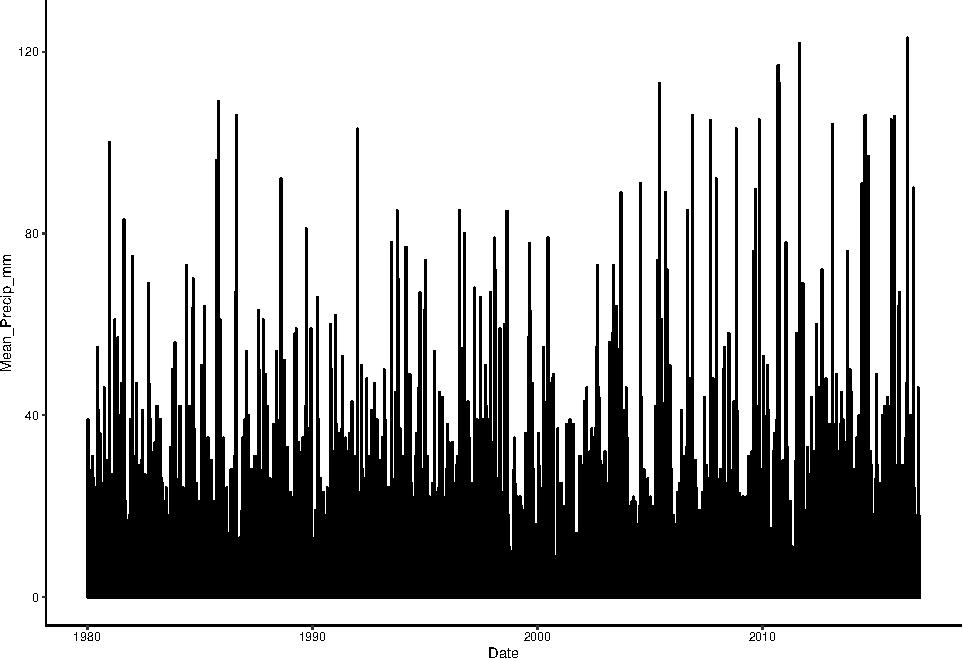
\includegraphics{Project_Template_TLK_files/figure-latex/initial plots-1.pdf}

\begin{Shaded}
\begin{Highlighting}[]
\CommentTok{\#plot total monthly precip data to see rough trend}
\FunctionTok{ggplot}\NormalTok{(Beaufort\_Clean, }\FunctionTok{aes}\NormalTok{(}\AttributeTok{x=}\NormalTok{Date, }\AttributeTok{y=}\NormalTok{sumMonthlyPrecip))}\SpecialCharTok{+}
  \FunctionTok{geom\_line}\NormalTok{()}\SpecialCharTok{+}
  \FunctionTok{geom\_smooth}\NormalTok{(}\AttributeTok{method =}\NormalTok{ lm) }
\end{Highlighting}
\end{Shaded}

\begin{verbatim}
## `geom_smooth()` using formula 'y ~ x'
\end{verbatim}

\begin{verbatim}
## Warning: Removed 9 rows containing non-finite values (stat_smooth).
\end{verbatim}

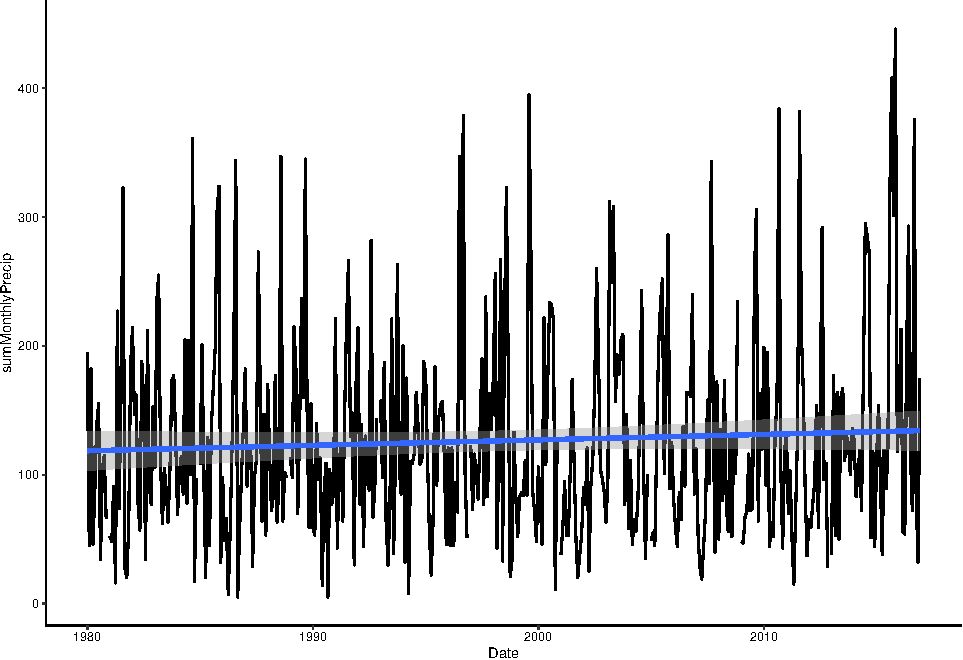
\includegraphics{Project_Template_TLK_files/figure-latex/initial plots-2.pdf}

\begin{Shaded}
\begin{Highlighting}[]
\FunctionTok{t.test}\NormalTok{(Beaufort\_RAW}\SpecialCharTok{$}\NormalTok{Mean\_Precip\_mm)}
\end{Highlighting}
\end{Shaded}

\begin{verbatim}
## 
##  One Sample t-test
## 
## data:  Beaufort_RAW$Mean_Precip_mm
## t = 43.492, df = 13504, p-value < 2.2e-16
## alternative hypothesis: true mean is not equal to 0
## 95 percent confidence interval:
##  3.953508 4.326684
## sample estimates:
## mean of x 
##  4.140096
\end{verbatim}

\begin{Shaded}
\begin{Highlighting}[]
\CommentTok{\#significant}

\CommentTok{\#Using Seasonal Mann{-}Kendall to look at trend excluding seasonality. Will be better than t{-}test, but we ar just running both just in case.}
\NormalTok{Beaufort\_RAW\_2}\OtherTok{\textless{}{-}}\NormalTok{Beaufort\_RAW}

\CommentTok{\#Used linear interpolation to fill missing data for precipitation data.}
\NormalTok{Beaufort\_RAW\_2}\SpecialCharTok{$}\NormalTok{Mean\_Precip\_mm}\OtherTok{\textless{}{-}}
  \FunctionTok{na.approx}\NormalTok{(Beaufort\_RAW\_2}\SpecialCharTok{$}\NormalTok{Mean\_Precip\_mm)}

\CommentTok{\#Created a time series analysis of the precipitation data at Beaufort.}
\NormalTok{firstday}\OtherTok{\textless{}{-}} \FunctionTok{day}\NormalTok{(}\FunctionTok{first}\NormalTok{(Beaufort\_RAW\_2}\SpecialCharTok{$}\NormalTok{Date))}
\NormalTok{firstmonth}\OtherTok{\textless{}{-}} \FunctionTok{month}\NormalTok{(}\FunctionTok{first}\NormalTok{(Beaufort\_RAW\_2}\SpecialCharTok{$}\NormalTok{Date))}
\NormalTok{firstyear}\OtherTok{\textless{}{-}} \FunctionTok{year}\NormalTok{(}\FunctionTok{first}\NormalTok{(Beaufort\_RAW\_2}\SpecialCharTok{$}\NormalTok{Date))}


\NormalTok{Beaufort\_TS}\OtherTok{\textless{}{-}} \FunctionTok{ts}\NormalTok{(Beaufort\_RAW\_2}\SpecialCharTok{$}\NormalTok{Mean\_Precip\_mm, }
                 \AttributeTok{start =} \FunctionTok{c}\NormalTok{(firstyear, firstmonth, firstday),}
                 \AttributeTok{frequency =} \DecValTok{365}\NormalTok{)}

\CommentTok{\#Decomposed the time series to see components.}
\NormalTok{Beaufort\_decompose}\OtherTok{\textless{}{-}} \FunctionTok{stl}\NormalTok{(Beaufort\_TS, }\AttributeTok{s.window =} \StringTok{"periodic"}\NormalTok{)}
\FunctionTok{plot}\NormalTok{(Beaufort\_decompose)}
\end{Highlighting}
\end{Shaded}

\includegraphics{Project_Template_TLK_files/figure-latex/t-test Overall\& Seasonal Mann-Kendall Ovearall-1.pdf}

\begin{Shaded}
\begin{Highlighting}[]
\CommentTok{\#Ran a seasonal Mann Kendall to see if there is a change in precipitation over the time of the data frame. Used seasonal Mann{-}Kendall to exclude seasonality of precipitation. }
\NormalTok{Beaufort.trend}\OtherTok{\textless{}{-}}\NormalTok{Kendall}\SpecialCharTok{::}\FunctionTok{SeasonalMannKendall}\NormalTok{(Beaufort\_TS)}
\NormalTok{Beaufort.trend}
\end{Highlighting}
\end{Shaded}

\begin{verbatim}
## tau = 0.0189, 2-sided pvalue =0.0056612
\end{verbatim}

\begin{Shaded}
\begin{Highlighting}[]
\CommentTok{\#Significant!}
\end{Highlighting}
\end{Shaded}

\begin{Shaded}
\begin{Highlighting}[]
\CommentTok{\#Here we are looking to see if there is a change in precipitation amount comparing two decades (1999{-}2006) \& (2007{-}2016)}
\FunctionTok{t.test}\NormalTok{(Beaufort\_early}\SpecialCharTok{$}\NormalTok{PrecipInches, Beaufort\_Late}\SpecialCharTok{$}\NormalTok{PrecipInches)}
\end{Highlighting}
\end{Shaded}

\begin{verbatim}
## 
##  Welch Two Sample t-test
## 
## data:  Beaufort_early$PrecipInches and Beaufort_Late$PrecipInches
## t = -0.64906, df = 7133.8, p-value = 0.5163
## alternative hypothesis: true difference in means is not equal to 0
## 95 percent confidence interval:
##  -0.02812072  0.01413102
## sample estimates:
## mean of x mean of y 
## 0.1627598 0.1697546
\end{verbatim}

\begin{Shaded}
\begin{Highlighting}[]
\CommentTok{\#not significant\textless{}{-} meaning precipitation amount not significantly different over the two decades}

\CommentTok{\#Here we compared the significant precipitation events for the two decades (1999{-}2006) \& (2007{-}2016).}
\FunctionTok{t.test}\NormalTok{(Beaufort\_early}\SpecialCharTok{$}\NormalTok{sigPrecip, Beaufort\_Late}\SpecialCharTok{$}\NormalTok{sigPrecip)}
\end{Highlighting}
\end{Shaded}

\begin{verbatim}
## 
##  Welch Two Sample t-test
## 
## data:  Beaufort_early$sigPrecip and Beaufort_Late$sigPrecip
## t = -2.7068, df = 5451.7, p-value = 0.006815
## alternative hypothesis: true difference in means is not equal to 0
## 95 percent confidence interval:
##  -0.028681849 -0.004586864
## sample estimates:
##   mean of x   mean of y 
## 0.005537589 0.022171945
\end{verbatim}

\begin{Shaded}
\begin{Highlighting}[]
\CommentTok{\#significant!\textless{}{-} There are more statistically significant 1 year precipitation events in later decade. }
\end{Highlighting}
\end{Shaded}

\begin{Shaded}
\begin{Highlighting}[]
\CommentTok{\#Will not include this in final....}

\CommentTok{\#Note: probably won\textquotesingle{}t include this because the data is seasonal data}
\FunctionTok{MannKendall}\NormalTok{(Beaufort\_early}\SpecialCharTok{$}\NormalTok{PrecipInches)}
\end{Highlighting}
\end{Shaded}

\begin{verbatim}
## tau = -0.00554, 2-sided pvalue =0.66022
\end{verbatim}

\begin{Shaded}
\begin{Highlighting}[]
\FunctionTok{MannKendall}\NormalTok{(Beaufort\_early}\SpecialCharTok{$}\NormalTok{sigPrecip)}
\end{Highlighting}
\end{Shaded}

\begin{verbatim}
## tau = 0.00613, 2-sided pvalue =0.65011
\end{verbatim}

\begin{Shaded}
\begin{Highlighting}[]
\CommentTok{\#neither are significant}

\FunctionTok{MannKendall}\NormalTok{(Beaufort\_Late}\SpecialCharTok{$}\NormalTok{PrecipInches)}
\end{Highlighting}
\end{Shaded}

\begin{verbatim}
## tau = 0.0638, 2-sided pvalue =0.00000035763
\end{verbatim}

\begin{Shaded}
\begin{Highlighting}[]
\CommentTok{\#significant}
\FunctionTok{MannKendall}\NormalTok{(Beaufort\_Late}\SpecialCharTok{$}\NormalTok{sigPrecip)}
\end{Highlighting}
\end{Shaded}

\begin{verbatim}
## tau = 0.00857, 2-sided pvalue =0.52552
\end{verbatim}

\begin{Shaded}
\begin{Highlighting}[]
\CommentTok{\#not significant}
\end{Highlighting}
\end{Shaded}

\begin{Shaded}
\begin{Highlighting}[]
\CommentTok{\#Dont think we need to keep this as it shows if precip is increasing in just this decade or not}
\NormalTok{Late\_full\_ts }\OtherTok{\textless{}{-}} \FunctionTok{ts}\NormalTok{(Beaufort\_Late}\SpecialCharTok{$}\NormalTok{PrecipInches, }\AttributeTok{start=} \FunctionTok{c}\NormalTok{(}\DecValTok{1}\NormalTok{,}\DecValTok{2007}\NormalTok{), }\AttributeTok{frequency =} \DecValTok{365}\NormalTok{)}
\FunctionTok{SeasonalMannKendall}\NormalTok{(Late\_full\_ts)}
\end{Highlighting}
\end{Shaded}

\begin{verbatim}
## WARNING: Error exit, tauk2. IFAULT =  12
## WARNING: Error exit, tauk2. IFAULT =  12
## WARNING: Error exit, tauk2. IFAULT =  12
## WARNING: Error exit, tauk2. IFAULT =  12
## WARNING: Error exit, tauk2. IFAULT =  12
## WARNING: Error exit, tauk2. IFAULT =  12
## WARNING: Error exit, tauk2. IFAULT =  12
## WARNING: Error exit, tauk2. IFAULT =  12
## WARNING: Error exit, tauk2. IFAULT =  12
## WARNING: Error exit, tauk2. IFAULT =  12
## WARNING: Error exit, tauk2. IFAULT =  12
## WARNING: Error exit, tauk2. IFAULT =  12
\end{verbatim}

\begin{verbatim}
## tau = 0.066, 2-sided pvalue =0.0000066885
\end{verbatim}

\begin{Shaded}
\begin{Highlighting}[]
\CommentTok{\#significant}

\CommentTok{\#Shouldn\textquotesingle{}t keep this}
\NormalTok{Late\_sig\_ts }\OtherTok{\textless{}{-}} \FunctionTok{ts}\NormalTok{(Beaufort\_Late}\SpecialCharTok{$}\NormalTok{sigPrecip, }\AttributeTok{start=} \FunctionTok{c}\NormalTok{(}\DecValTok{1}\NormalTok{,}\DecValTok{2007}\NormalTok{), }\AttributeTok{frequency =} \DecValTok{365}\NormalTok{)}
\FunctionTok{SeasonalMannKendall}\NormalTok{(Late\_sig\_ts)}
\end{Highlighting}
\end{Shaded}

\begin{verbatim}
## WARNING: Error exit, tauk2. IFAULT =  12
## WARNING: Error exit, tauk2. IFAULT =  12
## WARNING: Error exit, tauk2. IFAULT =  12
## WARNING: Error exit, tauk2. IFAULT =  12
## WARNING: Error exit, tauk2. IFAULT =  12
## WARNING: Error exit, tauk2. IFAULT =  12
## WARNING: Error exit, tauk2. IFAULT =  12
## WARNING: Error exit, tauk2. IFAULT =  12
## WARNING: Error exit, tauk2. IFAULT =  12
## WARNING: Error exit, tauk2. IFAULT =  12
## WARNING: Error exit, tauk2. IFAULT =  12
## WARNING: Error exit, tauk2. IFAULT =  12
## WARNING: Error exit, tauk2. IFAULT =  12
## WARNING: Error exit, tauk2. IFAULT =  12
## WARNING: Error exit, tauk2. IFAULT =  12
## WARNING: Error exit, tauk2. IFAULT =  12
## WARNING: Error exit, tauk2. IFAULT =  12
## WARNING: Error exit, tauk2. IFAULT =  12
## WARNING: Error exit, tauk2. IFAULT =  12
## WARNING: Error exit, tauk2. IFAULT =  12
## WARNING: Error exit, tauk2. IFAULT =  12
## WARNING: Error exit, tauk2. IFAULT =  12
## WARNING: Error exit, tauk2. IFAULT =  12
## WARNING: Error exit, tauk2. IFAULT =  12
## WARNING: Error exit, tauk2. IFAULT =  12
## WARNING: Error exit, tauk2. IFAULT =  12
## WARNING: Error exit, tauk2. IFAULT =  12
## WARNING: Error exit, tauk2. IFAULT =  12
## WARNING: Error exit, tauk2. IFAULT =  12
## WARNING: Error exit, tauk2. IFAULT =  12
## WARNING: Error exit, tauk2. IFAULT =  12
## WARNING: Error exit, tauk2. IFAULT =  12
## WARNING: Error exit, tauk2. IFAULT =  12
## WARNING: Error exit, tauk2. IFAULT =  12
## WARNING: Error exit, tauk2. IFAULT =  12
## WARNING: Error exit, tauk2. IFAULT =  12
## WARNING: Error exit, tauk2. IFAULT =  12
## WARNING: Error exit, tauk2. IFAULT =  12
## WARNING: Error exit, tauk2. IFAULT =  12
## WARNING: Error exit, tauk2. IFAULT =  12
## WARNING: Error exit, tauk2. IFAULT =  12
## WARNING: Error exit, tauk2. IFAULT =  12
## WARNING: Error exit, tauk2. IFAULT =  12
## WARNING: Error exit, tauk2. IFAULT =  12
## WARNING: Error exit, tauk2. IFAULT =  12
## WARNING: Error exit, tauk2. IFAULT =  12
## WARNING: Error exit, tauk2. IFAULT =  12
## WARNING: Error exit, tauk2. IFAULT =  12
## WARNING: Error exit, tauk2. IFAULT =  12
## WARNING: Error exit, tauk2. IFAULT =  12
## WARNING: Error exit, tauk2. IFAULT =  12
## WARNING: Error exit, tauk2. IFAULT =  12
## WARNING: Error exit, tauk2. IFAULT =  12
## WARNING: Error exit, tauk2. IFAULT =  12
## WARNING: Error exit, tauk2. IFAULT =  12
## WARNING: Error exit, tauk2. IFAULT =  12
## WARNING: Error exit, tauk2. IFAULT =  12
## WARNING: Error exit, tauk2. IFAULT =  12
## WARNING: Error exit, tauk2. IFAULT =  12
## WARNING: Error exit, tauk2. IFAULT =  12
## WARNING: Error exit, tauk2. IFAULT =  12
## WARNING: Error exit, tauk2. IFAULT =  12
## WARNING: Error exit, tauk2. IFAULT =  12
## WARNING: Error exit, tauk2. IFAULT =  12
## WARNING: Error exit, tauk2. IFAULT =  12
## WARNING: Error exit, tauk2. IFAULT =  12
## WARNING: Error exit, tauk2. IFAULT =  12
## WARNING: Error exit, tauk2. IFAULT =  12
## WARNING: Error exit, tauk2. IFAULT =  12
## WARNING: Error exit, tauk2. IFAULT =  12
## WARNING: Error exit, tauk2. IFAULT =  12
## WARNING: Error exit, tauk2. IFAULT =  12
## WARNING: Error exit, tauk2. IFAULT =  12
## WARNING: Error exit, tauk2. IFAULT =  12
## WARNING: Error exit, tauk2. IFAULT =  12
## WARNING: Error exit, tauk2. IFAULT =  12
## WARNING: Error exit, tauk2. IFAULT =  12
## WARNING: Error exit, tauk2. IFAULT =  12
## WARNING: Error exit, tauk2. IFAULT =  12
## WARNING: Error exit, tauk2. IFAULT =  12
## WARNING: Error exit, tauk2. IFAULT =  12
## WARNING: Error exit, tauk2. IFAULT =  12
## WARNING: Error exit, tauk2. IFAULT =  12
## WARNING: Error exit, tauk2. IFAULT =  12
## WARNING: Error exit, tauk2. IFAULT =  12
## WARNING: Error exit, tauk2. IFAULT =  12
## WARNING: Error exit, tauk2. IFAULT =  12
## WARNING: Error exit, tauk2. IFAULT =  12
## WARNING: Error exit, tauk2. IFAULT =  12
## WARNING: Error exit, tauk2. IFAULT =  12
## WARNING: Error exit, tauk2. IFAULT =  12
## WARNING: Error exit, tauk2. IFAULT =  12
## WARNING: Error exit, tauk2. IFAULT =  12
## WARNING: Error exit, tauk2. IFAULT =  12
## WARNING: Error exit, tauk2. IFAULT =  12
## WARNING: Error exit, tauk2. IFAULT =  12
## WARNING: Error exit, tauk2. IFAULT =  12
## WARNING: Error exit, tauk2. IFAULT =  12
## WARNING: Error exit, tauk2. IFAULT =  12
## WARNING: Error exit, tauk2. IFAULT =  12
## WARNING: Error exit, tauk2. IFAULT =  12
## WARNING: Error exit, tauk2. IFAULT =  12
## WARNING: Error exit, tauk2. IFAULT =  12
## WARNING: Error exit, tauk2. IFAULT =  12
## WARNING: Error exit, tauk2. IFAULT =  12
## WARNING: Error exit, tauk2. IFAULT =  12
## WARNING: Error exit, tauk2. IFAULT =  12
## WARNING: Error exit, tauk2. IFAULT =  12
## WARNING: Error exit, tauk2. IFAULT =  12
## WARNING: Error exit, tauk2. IFAULT =  12
## WARNING: Error exit, tauk2. IFAULT =  12
## WARNING: Error exit, tauk2. IFAULT =  12
## WARNING: Error exit, tauk2. IFAULT =  12
## WARNING: Error exit, tauk2. IFAULT =  12
## WARNING: Error exit, tauk2. IFAULT =  12
## WARNING: Error exit, tauk2. IFAULT =  12
## WARNING: Error exit, tauk2. IFAULT =  12
## WARNING: Error exit, tauk2. IFAULT =  12
## WARNING: Error exit, tauk2. IFAULT =  12
## WARNING: Error exit, tauk2. IFAULT =  12
## WARNING: Error exit, tauk2. IFAULT =  12
## WARNING: Error exit, tauk2. IFAULT =  12
## WARNING: Error exit, tauk2. IFAULT =  12
## WARNING: Error exit, tauk2. IFAULT =  12
## WARNING: Error exit, tauk2. IFAULT =  12
## WARNING: Error exit, tauk2. IFAULT =  12
## WARNING: Error exit, tauk2. IFAULT =  12
## WARNING: Error exit, tauk2. IFAULT =  12
## WARNING: Error exit, tauk2. IFAULT =  12
## WARNING: Error exit, tauk2. IFAULT =  12
## WARNING: Error exit, tauk2. IFAULT =  12
## WARNING: Error exit, tauk2. IFAULT =  12
## WARNING: Error exit, tauk2. IFAULT =  12
## WARNING: Error exit, tauk2. IFAULT =  12
## WARNING: Error exit, tauk2. IFAULT =  12
## WARNING: Error exit, tauk2. IFAULT =  12
## WARNING: Error exit, tauk2. IFAULT =  12
## WARNING: Error exit, tauk2. IFAULT =  12
## WARNING: Error exit, tauk2. IFAULT =  12
## WARNING: Error exit, tauk2. IFAULT =  12
## WARNING: Error exit, tauk2. IFAULT =  12
## WARNING: Error exit, tauk2. IFAULT =  12
## WARNING: Error exit, tauk2. IFAULT =  12
## WARNING: Error exit, tauk2. IFAULT =  12
## WARNING: Error exit, tauk2. IFAULT =  12
## WARNING: Error exit, tauk2. IFAULT =  12
## WARNING: Error exit, tauk2. IFAULT =  12
## WARNING: Error exit, tauk2. IFAULT =  12
## WARNING: Error exit, tauk2. IFAULT =  12
## WARNING: Error exit, tauk2. IFAULT =  12
## WARNING: Error exit, tauk2. IFAULT =  12
## WARNING: Error exit, tauk2. IFAULT =  12
## WARNING: Error exit, tauk2. IFAULT =  12
## WARNING: Error exit, tauk2. IFAULT =  12
## WARNING: Error exit, tauk2. IFAULT =  12
## WARNING: Error exit, tauk2. IFAULT =  12
## WARNING: Error exit, tauk2. IFAULT =  12
## WARNING: Error exit, tauk2. IFAULT =  12
## WARNING: Error exit, tauk2. IFAULT =  12
## WARNING: Error exit, tauk2. IFAULT =  12
## WARNING: Error exit, tauk2. IFAULT =  12
## WARNING: Error exit, tauk2. IFAULT =  12
## WARNING: Error exit, tauk2. IFAULT =  12
## WARNING: Error exit, tauk2. IFAULT =  12
## WARNING: Error exit, tauk2. IFAULT =  12
## WARNING: Error exit, tauk2. IFAULT =  12
## WARNING: Error exit, tauk2. IFAULT =  12
## WARNING: Error exit, tauk2. IFAULT =  12
## WARNING: Error exit, tauk2. IFAULT =  12
## WARNING: Error exit, tauk2. IFAULT =  12
## WARNING: Error exit, tauk2. IFAULT =  12
## WARNING: Error exit, tauk2. IFAULT =  12
## WARNING: Error exit, tauk2. IFAULT =  12
## WARNING: Error exit, tauk2. IFAULT =  12
## WARNING: Error exit, tauk2. IFAULT =  12
## WARNING: Error exit, tauk2. IFAULT =  12
## WARNING: Error exit, tauk2. IFAULT =  12
## WARNING: Error exit, tauk2. IFAULT =  12
## WARNING: Error exit, tauk2. IFAULT =  12
## WARNING: Error exit, tauk2. IFAULT =  12
## WARNING: Error exit, tauk2. IFAULT =  12
## WARNING: Error exit, tauk2. IFAULT =  12
## WARNING: Error exit, tauk2. IFAULT =  12
## WARNING: Error exit, tauk2. IFAULT =  12
## WARNING: Error exit, tauk2. IFAULT =  12
## WARNING: Error exit, tauk2. IFAULT =  12
## WARNING: Error exit, tauk2. IFAULT =  12
## WARNING: Error exit, tauk2. IFAULT =  12
## WARNING: Error exit, tauk2. IFAULT =  12
## WARNING: Error exit, tauk2. IFAULT =  12
## WARNING: Error exit, tauk2. IFAULT =  12
## WARNING: Error exit, tauk2. IFAULT =  12
## WARNING: Error exit, tauk2. IFAULT =  12
## WARNING: Error exit, tauk2. IFAULT =  12
## WARNING: Error exit, tauk2. IFAULT =  12
## WARNING: Error exit, tauk2. IFAULT =  12
## WARNING: Error exit, tauk2. IFAULT =  12
## WARNING: Error exit, tauk2. IFAULT =  12
## WARNING: Error exit, tauk2. IFAULT =  12
## WARNING: Error exit, tauk2. IFAULT =  12
## WARNING: Error exit, tauk2. IFAULT =  12
## WARNING: Error exit, tauk2. IFAULT =  12
## WARNING: Error exit, tauk2. IFAULT =  12
## WARNING: Error exit, tauk2. IFAULT =  12
## WARNING: Error exit, tauk2. IFAULT =  12
## WARNING: Error exit, tauk2. IFAULT =  12
## WARNING: Error exit, tauk2. IFAULT =  12
## WARNING: Error exit, tauk2. IFAULT =  12
## WARNING: Error exit, tauk2. IFAULT =  12
## WARNING: Error exit, tauk2. IFAULT =  12
## WARNING: Error exit, tauk2. IFAULT =  12
## WARNING: Error exit, tauk2. IFAULT =  12
## WARNING: Error exit, tauk2. IFAULT =  12
## WARNING: Error exit, tauk2. IFAULT =  12
## WARNING: Error exit, tauk2. IFAULT =  12
## WARNING: Error exit, tauk2. IFAULT =  12
## WARNING: Error exit, tauk2. IFAULT =  12
## WARNING: Error exit, tauk2. IFAULT =  12
## WARNING: Error exit, tauk2. IFAULT =  12
## WARNING: Error exit, tauk2. IFAULT =  12
## WARNING: Error exit, tauk2. IFAULT =  12
## WARNING: Error exit, tauk2. IFAULT =  12
## WARNING: Error exit, tauk2. IFAULT =  12
## WARNING: Error exit, tauk2. IFAULT =  12
## WARNING: Error exit, tauk2. IFAULT =  12
## WARNING: Error exit, tauk2. IFAULT =  12
## WARNING: Error exit, tauk2. IFAULT =  12
## WARNING: Error exit, tauk2. IFAULT =  12
## WARNING: Error exit, tauk2. IFAULT =  12
## WARNING: Error exit, tauk2. IFAULT =  12
## WARNING: Error exit, tauk2. IFAULT =  12
## WARNING: Error exit, tauk2. IFAULT =  12
## WARNING: Error exit, tauk2. IFAULT =  12
## WARNING: Error exit, tauk2. IFAULT =  12
## WARNING: Error exit, tauk2. IFAULT =  12
## WARNING: Error exit, tauk2. IFAULT =  12
## WARNING: Error exit, tauk2. IFAULT =  12
## WARNING: Error exit, tauk2. IFAULT =  12
## WARNING: Error exit, tauk2. IFAULT =  12
## WARNING: Error exit, tauk2. IFAULT =  12
## WARNING: Error exit, tauk2. IFAULT =  12
## WARNING: Error exit, tauk2. IFAULT =  12
## WARNING: Error exit, tauk2. IFAULT =  12
## WARNING: Error exit, tauk2. IFAULT =  12
## WARNING: Error exit, tauk2. IFAULT =  12
## WARNING: Error exit, tauk2. IFAULT =  12
## WARNING: Error exit, tauk2. IFAULT =  12
## WARNING: Error exit, tauk2. IFAULT =  12
## WARNING: Error exit, tauk2. IFAULT =  12
## WARNING: Error exit, tauk2. IFAULT =  12
## WARNING: Error exit, tauk2. IFAULT =  12
## WARNING: Error exit, tauk2. IFAULT =  12
## WARNING: Error exit, tauk2. IFAULT =  12
## WARNING: Error exit, tauk2. IFAULT =  12
## WARNING: Error exit, tauk2. IFAULT =  12
## WARNING: Error exit, tauk2. IFAULT =  12
## WARNING: Error exit, tauk2. IFAULT =  12
## WARNING: Error exit, tauk2. IFAULT =  12
## WARNING: Error exit, tauk2. IFAULT =  12
## WARNING: Error exit, tauk2. IFAULT =  12
## WARNING: Error exit, tauk2. IFAULT =  12
## WARNING: Error exit, tauk2. IFAULT =  12
## WARNING: Error exit, tauk2. IFAULT =  12
## WARNING: Error exit, tauk2. IFAULT =  12
## WARNING: Error exit, tauk2. IFAULT =  12
## WARNING: Error exit, tauk2. IFAULT =  12
## WARNING: Error exit, tauk2. IFAULT =  12
## WARNING: Error exit, tauk2. IFAULT =  12
## WARNING: Error exit, tauk2. IFAULT =  12
## WARNING: Error exit, tauk2. IFAULT =  12
## WARNING: Error exit, tauk2. IFAULT =  12
## WARNING: Error exit, tauk2. IFAULT =  12
## WARNING: Error exit, tauk2. IFAULT =  12
## WARNING: Error exit, tauk2. IFAULT =  12
## WARNING: Error exit, tauk2. IFAULT =  12
## WARNING: Error exit, tauk2. IFAULT =  12
## WARNING: Error exit, tauk2. IFAULT =  12
## WARNING: Error exit, tauk2. IFAULT =  12
## WARNING: Error exit, tauk2. IFAULT =  12
## WARNING: Error exit, tauk2. IFAULT =  12
## WARNING: Error exit, tauk2. IFAULT =  12
## WARNING: Error exit, tauk2. IFAULT =  12
## WARNING: Error exit, tauk2. IFAULT =  12
## WARNING: Error exit, tauk2. IFAULT =  12
## WARNING: Error exit, tauk2. IFAULT =  12
## WARNING: Error exit, tauk2. IFAULT =  12
## WARNING: Error exit, tauk2. IFAULT =  12
## WARNING: Error exit, tauk2. IFAULT =  12
## WARNING: Error exit, tauk2. IFAULT =  12
## WARNING: Error exit, tauk2. IFAULT =  12
## WARNING: Error exit, tauk2. IFAULT =  12
## WARNING: Error exit, tauk2. IFAULT =  12
## WARNING: Error exit, tauk2. IFAULT =  12
## WARNING: Error exit, tauk2. IFAULT =  12
## WARNING: Error exit, tauk2. IFAULT =  12
## WARNING: Error exit, tauk2. IFAULT =  12
## WARNING: Error exit, tauk2. IFAULT =  12
## WARNING: Error exit, tauk2. IFAULT =  12
## WARNING: Error exit, tauk2. IFAULT =  12
## WARNING: Error exit, tauk2. IFAULT =  12
## WARNING: Error exit, tauk2. IFAULT =  12
## WARNING: Error exit, tauk2. IFAULT =  12
## WARNING: Error exit, tauk2. IFAULT =  12
## WARNING: Error exit, tauk2. IFAULT =  12
## WARNING: Error exit, tauk2. IFAULT =  12
## WARNING: Error exit, tauk2. IFAULT =  12
## WARNING: Error exit, tauk2. IFAULT =  12
## WARNING: Error exit, tauk2. IFAULT =  12
## WARNING: Error exit, tauk2. IFAULT =  12
## WARNING: Error exit, tauk2. IFAULT =  12
## WARNING: Error exit, tauk2. IFAULT =  12
## WARNING: Error exit, tauk2. IFAULT =  12
## WARNING: Error exit, tauk2. IFAULT =  12
## WARNING: Error exit, tauk2. IFAULT =  12
## WARNING: Error exit, tauk2. IFAULT =  12
## WARNING: Error exit, tauk2. IFAULT =  12
## WARNING: Error exit, tauk2. IFAULT =  12
## WARNING: Error exit, tauk2. IFAULT =  12
## WARNING: Error exit, tauk2. IFAULT =  12
## WARNING: Error exit, tauk2. IFAULT =  12
## WARNING: Error exit, tauk2. IFAULT =  12
## WARNING: Error exit, tauk2. IFAULT =  12
## WARNING: Error exit, tauk2. IFAULT =  12
## WARNING: Error exit, tauk2. IFAULT =  12
## WARNING: Error exit, tauk2. IFAULT =  12
## WARNING: Error exit, tauk2. IFAULT =  12
## WARNING: Error exit, tauk2. IFAULT =  12
## WARNING: Error exit, tauk2. IFAULT =  12
## WARNING: Error exit, tauk2. IFAULT =  12
## WARNING: Error exit, tauk2. IFAULT =  12
## WARNING: Error exit, tauk2. IFAULT =  12
## WARNING: Error exit, tauk2. IFAULT =  12
## WARNING: Error exit, tauk2. IFAULT =  12
## WARNING: Error exit, tauk2. IFAULT =  12
## WARNING: Error exit, tauk2. IFAULT =  12
## WARNING: Error exit, tauk2. IFAULT =  12
## WARNING: Error exit, tauk2. IFAULT =  12
## WARNING: Error exit, tauk2. IFAULT =  12
## WARNING: Error exit, tauk2. IFAULT =  12
## WARNING: Error exit, tauk2. IFAULT =  12
## WARNING: Error exit, tauk2. IFAULT =  12
## WARNING: Error exit, tauk2. IFAULT =  12
## WARNING: Error exit, tauk2. IFAULT =  12
## WARNING: Error exit, tauk2. IFAULT =  12
## WARNING: Error exit, tauk2. IFAULT =  12
## WARNING: Error exit, tauk2. IFAULT =  12
## WARNING: Error exit, tauk2. IFAULT =  12
## WARNING: Error exit, tauk2. IFAULT =  12
## WARNING: Error exit, tauk2. IFAULT =  12
\end{verbatim}

\begin{verbatim}
## tau = 0.0243, 2-sided pvalue =0.7341
\end{verbatim}

\begin{Shaded}
\begin{Highlighting}[]
\CommentTok{\#not significant}

\CommentTok{\#Dont think we need to keep this as it shows if precip is increasing in just this decade or not}
\NormalTok{Early\_full\_ts }\OtherTok{\textless{}{-}} \FunctionTok{ts}\NormalTok{(Beaufort\_early}\SpecialCharTok{$}\NormalTok{PrecipInches, }\AttributeTok{start =} \FunctionTok{c}\NormalTok{(}\DecValTok{1}\NormalTok{,}\DecValTok{1997}\NormalTok{), }\AttributeTok{frequency =} \DecValTok{365}\NormalTok{)}
\FunctionTok{SeasonalMannKendall}\NormalTok{(Early\_full\_ts)}
\end{Highlighting}
\end{Shaded}

\begin{verbatim}
## WARNING: Error exit, tauk2. IFAULT =  12
## WARNING: Error exit, tauk2. IFAULT =  12
## WARNING: Error exit, tauk2. IFAULT =  12
## WARNING: Error exit, tauk2. IFAULT =  12
## WARNING: Error exit, tauk2. IFAULT =  12
## WARNING: Error exit, tauk2. IFAULT =  12
## WARNING: Error exit, tauk2. IFAULT =  12
## WARNING: Error exit, tauk2. IFAULT =  12
## WARNING: Error exit, tauk2. IFAULT =  12
## WARNING: Error exit, tauk2. IFAULT =  12
## WARNING: Error exit, tauk2. IFAULT =  12
## WARNING: Error exit, tauk2. IFAULT =  12
## WARNING: Error exit, tauk2. IFAULT =  12
## WARNING: Error exit, tauk2. IFAULT =  12
## WARNING: Error exit, tauk2. IFAULT =  12
\end{verbatim}

\begin{verbatim}
## tau = -0.00305, 2-sided pvalue =0.83608
\end{verbatim}

\begin{Shaded}
\begin{Highlighting}[]
\CommentTok{\#not significant}

\CommentTok{\#will not keep this too }
\NormalTok{Early\_sig\_ts }\OtherTok{\textless{}{-}} \FunctionTok{ts}\NormalTok{(Beaufort\_early}\SpecialCharTok{$}\NormalTok{sigPrecip, }\AttributeTok{start =} \FunctionTok{c}\NormalTok{(}\DecValTok{1}\NormalTok{,}\DecValTok{1997}\NormalTok{), }\AttributeTok{frequency =} \DecValTok{365}\NormalTok{)}
\FunctionTok{SeasonalMannKendall}\NormalTok{(Early\_sig\_ts)}
\end{Highlighting}
\end{Shaded}

\begin{verbatim}
## WARNING: Error exit, tauk2. IFAULT =  12
## WARNING: Error exit, tauk2. IFAULT =  12
## WARNING: Error exit, tauk2. IFAULT =  12
## WARNING: Error exit, tauk2. IFAULT =  12
## WARNING: Error exit, tauk2. IFAULT =  12
## WARNING: Error exit, tauk2. IFAULT =  12
## WARNING: Error exit, tauk2. IFAULT =  12
## WARNING: Error exit, tauk2. IFAULT =  12
## WARNING: Error exit, tauk2. IFAULT =  12
## WARNING: Error exit, tauk2. IFAULT =  12
## WARNING: Error exit, tauk2. IFAULT =  12
## WARNING: Error exit, tauk2. IFAULT =  12
## WARNING: Error exit, tauk2. IFAULT =  12
## WARNING: Error exit, tauk2. IFAULT =  12
## WARNING: Error exit, tauk2. IFAULT =  12
## WARNING: Error exit, tauk2. IFAULT =  12
## WARNING: Error exit, tauk2. IFAULT =  12
## WARNING: Error exit, tauk2. IFAULT =  12
## WARNING: Error exit, tauk2. IFAULT =  12
## WARNING: Error exit, tauk2. IFAULT =  12
## WARNING: Error exit, tauk2. IFAULT =  12
## WARNING: Error exit, tauk2. IFAULT =  12
## WARNING: Error exit, tauk2. IFAULT =  12
## WARNING: Error exit, tauk2. IFAULT =  12
## WARNING: Error exit, tauk2. IFAULT =  12
## WARNING: Error exit, tauk2. IFAULT =  12
## WARNING: Error exit, tauk2. IFAULT =  12
## WARNING: Error exit, tauk2. IFAULT =  12
## WARNING: Error exit, tauk2. IFAULT =  12
## WARNING: Error exit, tauk2. IFAULT =  12
## WARNING: Error exit, tauk2. IFAULT =  12
## WARNING: Error exit, tauk2. IFAULT =  12
## WARNING: Error exit, tauk2. IFAULT =  12
## WARNING: Error exit, tauk2. IFAULT =  12
## WARNING: Error exit, tauk2. IFAULT =  12
## WARNING: Error exit, tauk2. IFAULT =  12
## WARNING: Error exit, tauk2. IFAULT =  12
## WARNING: Error exit, tauk2. IFAULT =  12
## WARNING: Error exit, tauk2. IFAULT =  12
## WARNING: Error exit, tauk2. IFAULT =  12
## WARNING: Error exit, tauk2. IFAULT =  12
## WARNING: Error exit, tauk2. IFAULT =  12
## WARNING: Error exit, tauk2. IFAULT =  12
## WARNING: Error exit, tauk2. IFAULT =  12
## WARNING: Error exit, tauk2. IFAULT =  12
## WARNING: Error exit, tauk2. IFAULT =  12
## WARNING: Error exit, tauk2. IFAULT =  12
## WARNING: Error exit, tauk2. IFAULT =  12
## WARNING: Error exit, tauk2. IFAULT =  12
## WARNING: Error exit, tauk2. IFAULT =  12
## WARNING: Error exit, tauk2. IFAULT =  12
## WARNING: Error exit, tauk2. IFAULT =  12
## WARNING: Error exit, tauk2. IFAULT =  12
## WARNING: Error exit, tauk2. IFAULT =  12
## WARNING: Error exit, tauk2. IFAULT =  12
## WARNING: Error exit, tauk2. IFAULT =  12
## WARNING: Error exit, tauk2. IFAULT =  12
## WARNING: Error exit, tauk2. IFAULT =  12
## WARNING: Error exit, tauk2. IFAULT =  12
## WARNING: Error exit, tauk2. IFAULT =  12
## WARNING: Error exit, tauk2. IFAULT =  12
## WARNING: Error exit, tauk2. IFAULT =  12
## WARNING: Error exit, tauk2. IFAULT =  12
## WARNING: Error exit, tauk2. IFAULT =  12
## WARNING: Error exit, tauk2. IFAULT =  12
## WARNING: Error exit, tauk2. IFAULT =  12
## WARNING: Error exit, tauk2. IFAULT =  12
## WARNING: Error exit, tauk2. IFAULT =  12
## WARNING: Error exit, tauk2. IFAULT =  12
## WARNING: Error exit, tauk2. IFAULT =  12
## WARNING: Error exit, tauk2. IFAULT =  12
## WARNING: Error exit, tauk2. IFAULT =  12
## WARNING: Error exit, tauk2. IFAULT =  12
## WARNING: Error exit, tauk2. IFAULT =  12
## WARNING: Error exit, tauk2. IFAULT =  12
## WARNING: Error exit, tauk2. IFAULT =  12
## WARNING: Error exit, tauk2. IFAULT =  12
## WARNING: Error exit, tauk2. IFAULT =  12
## WARNING: Error exit, tauk2. IFAULT =  12
## WARNING: Error exit, tauk2. IFAULT =  12
## WARNING: Error exit, tauk2. IFAULT =  12
## WARNING: Error exit, tauk2. IFAULT =  12
## WARNING: Error exit, tauk2. IFAULT =  12
## WARNING: Error exit, tauk2. IFAULT =  12
## WARNING: Error exit, tauk2. IFAULT =  12
## WARNING: Error exit, tauk2. IFAULT =  12
## WARNING: Error exit, tauk2. IFAULT =  12
## WARNING: Error exit, tauk2. IFAULT =  12
## WARNING: Error exit, tauk2. IFAULT =  12
## WARNING: Error exit, tauk2. IFAULT =  12
## WARNING: Error exit, tauk2. IFAULT =  12
## WARNING: Error exit, tauk2. IFAULT =  12
## WARNING: Error exit, tauk2. IFAULT =  12
## WARNING: Error exit, tauk2. IFAULT =  12
## WARNING: Error exit, tauk2. IFAULT =  12
## WARNING: Error exit, tauk2. IFAULT =  12
## WARNING: Error exit, tauk2. IFAULT =  12
## WARNING: Error exit, tauk2. IFAULT =  12
## WARNING: Error exit, tauk2. IFAULT =  12
## WARNING: Error exit, tauk2. IFAULT =  12
## WARNING: Error exit, tauk2. IFAULT =  12
## WARNING: Error exit, tauk2. IFAULT =  12
## WARNING: Error exit, tauk2. IFAULT =  12
## WARNING: Error exit, tauk2. IFAULT =  12
## WARNING: Error exit, tauk2. IFAULT =  12
## WARNING: Error exit, tauk2. IFAULT =  12
## WARNING: Error exit, tauk2. IFAULT =  12
## WARNING: Error exit, tauk2. IFAULT =  12
## WARNING: Error exit, tauk2. IFAULT =  12
## WARNING: Error exit, tauk2. IFAULT =  12
## WARNING: Error exit, tauk2. IFAULT =  12
## WARNING: Error exit, tauk2. IFAULT =  12
## WARNING: Error exit, tauk2. IFAULT =  12
## WARNING: Error exit, tauk2. IFAULT =  12
## WARNING: Error exit, tauk2. IFAULT =  12
## WARNING: Error exit, tauk2. IFAULT =  12
## WARNING: Error exit, tauk2. IFAULT =  12
## WARNING: Error exit, tauk2. IFAULT =  12
## WARNING: Error exit, tauk2. IFAULT =  12
## WARNING: Error exit, tauk2. IFAULT =  12
## WARNING: Error exit, tauk2. IFAULT =  12
## WARNING: Error exit, tauk2. IFAULT =  12
## WARNING: Error exit, tauk2. IFAULT =  12
## WARNING: Error exit, tauk2. IFAULT =  12
## WARNING: Error exit, tauk2. IFAULT =  12
## WARNING: Error exit, tauk2. IFAULT =  12
## WARNING: Error exit, tauk2. IFAULT =  12
## WARNING: Error exit, tauk2. IFAULT =  12
## WARNING: Error exit, tauk2. IFAULT =  12
## WARNING: Error exit, tauk2. IFAULT =  12
## WARNING: Error exit, tauk2. IFAULT =  12
## WARNING: Error exit, tauk2. IFAULT =  12
## WARNING: Error exit, tauk2. IFAULT =  12
## WARNING: Error exit, tauk2. IFAULT =  12
## WARNING: Error exit, tauk2. IFAULT =  12
## WARNING: Error exit, tauk2. IFAULT =  12
## WARNING: Error exit, tauk2. IFAULT =  12
## WARNING: Error exit, tauk2. IFAULT =  12
## WARNING: Error exit, tauk2. IFAULT =  12
## WARNING: Error exit, tauk2. IFAULT =  12
## WARNING: Error exit, tauk2. IFAULT =  12
## WARNING: Error exit, tauk2. IFAULT =  12
## WARNING: Error exit, tauk2. IFAULT =  12
## WARNING: Error exit, tauk2. IFAULT =  12
## WARNING: Error exit, tauk2. IFAULT =  12
## WARNING: Error exit, tauk2. IFAULT =  12
## WARNING: Error exit, tauk2. IFAULT =  12
## WARNING: Error exit, tauk2. IFAULT =  12
## WARNING: Error exit, tauk2. IFAULT =  12
## WARNING: Error exit, tauk2. IFAULT =  12
## WARNING: Error exit, tauk2. IFAULT =  12
## WARNING: Error exit, tauk2. IFAULT =  12
## WARNING: Error exit, tauk2. IFAULT =  12
## WARNING: Error exit, tauk2. IFAULT =  12
## WARNING: Error exit, tauk2. IFAULT =  12
## WARNING: Error exit, tauk2. IFAULT =  12
## WARNING: Error exit, tauk2. IFAULT =  12
## WARNING: Error exit, tauk2. IFAULT =  12
## WARNING: Error exit, tauk2. IFAULT =  12
## WARNING: Error exit, tauk2. IFAULT =  12
## WARNING: Error exit, tauk2. IFAULT =  12
## WARNING: Error exit, tauk2. IFAULT =  12
## WARNING: Error exit, tauk2. IFAULT =  12
## WARNING: Error exit, tauk2. IFAULT =  12
## WARNING: Error exit, tauk2. IFAULT =  12
## WARNING: Error exit, tauk2. IFAULT =  12
## WARNING: Error exit, tauk2. IFAULT =  12
## WARNING: Error exit, tauk2. IFAULT =  12
## WARNING: Error exit, tauk2. IFAULT =  12
## WARNING: Error exit, tauk2. IFAULT =  12
## WARNING: Error exit, tauk2. IFAULT =  12
## WARNING: Error exit, tauk2. IFAULT =  12
## WARNING: Error exit, tauk2. IFAULT =  12
## WARNING: Error exit, tauk2. IFAULT =  12
## WARNING: Error exit, tauk2. IFAULT =  12
## WARNING: Error exit, tauk2. IFAULT =  12
## WARNING: Error exit, tauk2. IFAULT =  12
## WARNING: Error exit, tauk2. IFAULT =  12
## WARNING: Error exit, tauk2. IFAULT =  12
## WARNING: Error exit, tauk2. IFAULT =  12
## WARNING: Error exit, tauk2. IFAULT =  12
## WARNING: Error exit, tauk2. IFAULT =  12
## WARNING: Error exit, tauk2. IFAULT =  12
## WARNING: Error exit, tauk2. IFAULT =  12
## WARNING: Error exit, tauk2. IFAULT =  12
## WARNING: Error exit, tauk2. IFAULT =  12
## WARNING: Error exit, tauk2. IFAULT =  12
## WARNING: Error exit, tauk2. IFAULT =  12
## WARNING: Error exit, tauk2. IFAULT =  12
## WARNING: Error exit, tauk2. IFAULT =  12
## WARNING: Error exit, tauk2. IFAULT =  12
## WARNING: Error exit, tauk2. IFAULT =  12
## WARNING: Error exit, tauk2. IFAULT =  12
## WARNING: Error exit, tauk2. IFAULT =  12
## WARNING: Error exit, tauk2. IFAULT =  12
## WARNING: Error exit, tauk2. IFAULT =  12
## WARNING: Error exit, tauk2. IFAULT =  12
## WARNING: Error exit, tauk2. IFAULT =  12
## WARNING: Error exit, tauk2. IFAULT =  12
## WARNING: Error exit, tauk2. IFAULT =  12
## WARNING: Error exit, tauk2. IFAULT =  12
## WARNING: Error exit, tauk2. IFAULT =  12
## WARNING: Error exit, tauk2. IFAULT =  12
## WARNING: Error exit, tauk2. IFAULT =  12
## WARNING: Error exit, tauk2. IFAULT =  12
## WARNING: Error exit, tauk2. IFAULT =  12
## WARNING: Error exit, tauk2. IFAULT =  12
## WARNING: Error exit, tauk2. IFAULT =  12
## WARNING: Error exit, tauk2. IFAULT =  12
## WARNING: Error exit, tauk2. IFAULT =  12
## WARNING: Error exit, tauk2. IFAULT =  12
## WARNING: Error exit, tauk2. IFAULT =  12
## WARNING: Error exit, tauk2. IFAULT =  12
## WARNING: Error exit, tauk2. IFAULT =  12
## WARNING: Error exit, tauk2. IFAULT =  12
## WARNING: Error exit, tauk2. IFAULT =  12
## WARNING: Error exit, tauk2. IFAULT =  12
## WARNING: Error exit, tauk2. IFAULT =  12
## WARNING: Error exit, tauk2. IFAULT =  12
## WARNING: Error exit, tauk2. IFAULT =  12
## WARNING: Error exit, tauk2. IFAULT =  12
## WARNING: Error exit, tauk2. IFAULT =  12
## WARNING: Error exit, tauk2. IFAULT =  12
## WARNING: Error exit, tauk2. IFAULT =  12
## WARNING: Error exit, tauk2. IFAULT =  12
## WARNING: Error exit, tauk2. IFAULT =  12
## WARNING: Error exit, tauk2. IFAULT =  12
## WARNING: Error exit, tauk2. IFAULT =  12
## WARNING: Error exit, tauk2. IFAULT =  12
## WARNING: Error exit, tauk2. IFAULT =  12
## WARNING: Error exit, tauk2. IFAULT =  12
## WARNING: Error exit, tauk2. IFAULT =  12
## WARNING: Error exit, tauk2. IFAULT =  12
## WARNING: Error exit, tauk2. IFAULT =  12
## WARNING: Error exit, tauk2. IFAULT =  12
## WARNING: Error exit, tauk2. IFAULT =  12
## WARNING: Error exit, tauk2. IFAULT =  12
## WARNING: Error exit, tauk2. IFAULT =  12
## WARNING: Error exit, tauk2. IFAULT =  12
## WARNING: Error exit, tauk2. IFAULT =  12
## WARNING: Error exit, tauk2. IFAULT =  12
## WARNING: Error exit, tauk2. IFAULT =  12
## WARNING: Error exit, tauk2. IFAULT =  12
## WARNING: Error exit, tauk2. IFAULT =  12
## WARNING: Error exit, tauk2. IFAULT =  12
## WARNING: Error exit, tauk2. IFAULT =  12
## WARNING: Error exit, tauk2. IFAULT =  12
## WARNING: Error exit, tauk2. IFAULT =  12
## WARNING: Error exit, tauk2. IFAULT =  12
## WARNING: Error exit, tauk2. IFAULT =  12
## WARNING: Error exit, tauk2. IFAULT =  12
## WARNING: Error exit, tauk2. IFAULT =  12
## WARNING: Error exit, tauk2. IFAULT =  12
## WARNING: Error exit, tauk2. IFAULT =  12
## WARNING: Error exit, tauk2. IFAULT =  12
## WARNING: Error exit, tauk2. IFAULT =  12
## WARNING: Error exit, tauk2. IFAULT =  12
## WARNING: Error exit, tauk2. IFAULT =  12
## WARNING: Error exit, tauk2. IFAULT =  12
## WARNING: Error exit, tauk2. IFAULT =  12
## WARNING: Error exit, tauk2. IFAULT =  12
## WARNING: Error exit, tauk2. IFAULT =  12
## WARNING: Error exit, tauk2. IFAULT =  12
## WARNING: Error exit, tauk2. IFAULT =  12
## WARNING: Error exit, tauk2. IFAULT =  12
## WARNING: Error exit, tauk2. IFAULT =  12
## WARNING: Error exit, tauk2. IFAULT =  12
## WARNING: Error exit, tauk2. IFAULT =  12
## WARNING: Error exit, tauk2. IFAULT =  12
## WARNING: Error exit, tauk2. IFAULT =  12
## WARNING: Error exit, tauk2. IFAULT =  12
## WARNING: Error exit, tauk2. IFAULT =  12
## WARNING: Error exit, tauk2. IFAULT =  12
## WARNING: Error exit, tauk2. IFAULT =  12
## WARNING: Error exit, tauk2. IFAULT =  12
## WARNING: Error exit, tauk2. IFAULT =  12
## WARNING: Error exit, tauk2. IFAULT =  12
## WARNING: Error exit, tauk2. IFAULT =  12
## WARNING: Error exit, tauk2. IFAULT =  12
## WARNING: Error exit, tauk2. IFAULT =  12
## WARNING: Error exit, tauk2. IFAULT =  12
## WARNING: Error exit, tauk2. IFAULT =  12
## WARNING: Error exit, tauk2. IFAULT =  12
## WARNING: Error exit, tauk2. IFAULT =  12
## WARNING: Error exit, tauk2. IFAULT =  12
## WARNING: Error exit, tauk2. IFAULT =  12
## WARNING: Error exit, tauk2. IFAULT =  12
## WARNING: Error exit, tauk2. IFAULT =  12
## WARNING: Error exit, tauk2. IFAULT =  12
## WARNING: Error exit, tauk2. IFAULT =  12
## WARNING: Error exit, tauk2. IFAULT =  12
## WARNING: Error exit, tauk2. IFAULT =  12
## WARNING: Error exit, tauk2. IFAULT =  12
## WARNING: Error exit, tauk2. IFAULT =  12
## WARNING: Error exit, tauk2. IFAULT =  12
## WARNING: Error exit, tauk2. IFAULT =  12
## WARNING: Error exit, tauk2. IFAULT =  12
## WARNING: Error exit, tauk2. IFAULT =  12
## WARNING: Error exit, tauk2. IFAULT =  12
## WARNING: Error exit, tauk2. IFAULT =  12
## WARNING: Error exit, tauk2. IFAULT =  12
## WARNING: Error exit, tauk2. IFAULT =  12
## WARNING: Error exit, tauk2. IFAULT =  12
## WARNING: Error exit, tauk2. IFAULT =  12
## WARNING: Error exit, tauk2. IFAULT =  12
## WARNING: Error exit, tauk2. IFAULT =  12
## WARNING: Error exit, tauk2. IFAULT =  12
## WARNING: Error exit, tauk2. IFAULT =  12
## WARNING: Error exit, tauk2. IFAULT =  12
## WARNING: Error exit, tauk2. IFAULT =  12
## WARNING: Error exit, tauk2. IFAULT =  12
## WARNING: Error exit, tauk2. IFAULT =  12
## WARNING: Error exit, tauk2. IFAULT =  12
## WARNING: Error exit, tauk2. IFAULT =  12
## WARNING: Error exit, tauk2. IFAULT =  12
## WARNING: Error exit, tauk2. IFAULT =  12
## WARNING: Error exit, tauk2. IFAULT =  12
## WARNING: Error exit, tauk2. IFAULT =  12
## WARNING: Error exit, tauk2. IFAULT =  12
## WARNING: Error exit, tauk2. IFAULT =  12
## WARNING: Error exit, tauk2. IFAULT =  12
## WARNING: Error exit, tauk2. IFAULT =  12
## WARNING: Error exit, tauk2. IFAULT =  12
## WARNING: Error exit, tauk2. IFAULT =  12
## WARNING: Error exit, tauk2. IFAULT =  12
## WARNING: Error exit, tauk2. IFAULT =  12
## WARNING: Error exit, tauk2. IFAULT =  12
## WARNING: Error exit, tauk2. IFAULT =  12
## WARNING: Error exit, tauk2. IFAULT =  12
## WARNING: Error exit, tauk2. IFAULT =  12
## WARNING: Error exit, tauk2. IFAULT =  12
## WARNING: Error exit, tauk2. IFAULT =  12
## WARNING: Error exit, tauk2. IFAULT =  12
## WARNING: Error exit, tauk2. IFAULT =  12
## WARNING: Error exit, tauk2. IFAULT =  12
## WARNING: Error exit, tauk2. IFAULT =  12
## WARNING: Error exit, tauk2. IFAULT =  12
## WARNING: Error exit, tauk2. IFAULT =  12
## WARNING: Error exit, tauk2. IFAULT =  12
## WARNING: Error exit, tauk2. IFAULT =  12
## WARNING: Error exit, tauk2. IFAULT =  12
## WARNING: Error exit, tauk2. IFAULT =  12
## WARNING: Error exit, tauk2. IFAULT =  12
## WARNING: Error exit, tauk2. IFAULT =  12
## WARNING: Error exit, tauk2. IFAULT =  12
## WARNING: Error exit, tauk2. IFAULT =  12
## WARNING: Error exit, tauk2. IFAULT =  12
## WARNING: Error exit, tauk2. IFAULT =  12
## WARNING: Error exit, tauk2. IFAULT =  12
## WARNING: Error exit, tauk2. IFAULT =  12
## WARNING: Error exit, tauk2. IFAULT =  12
## WARNING: Error exit, tauk2. IFAULT =  12
## WARNING: Error exit, tauk2. IFAULT =  12
## WARNING: Error exit, tauk2. IFAULT =  12
## WARNING: Error exit, tauk2. IFAULT =  12
## WARNING: Error exit, tauk2. IFAULT =  12
## WARNING: Error exit, tauk2. IFAULT =  12
## WARNING: Error exit, tauk2. IFAULT =  12
## WARNING: Error exit, tauk2. IFAULT =  12
## WARNING: Error exit, tauk2. IFAULT =  12
## WARNING: Error exit, tauk2. IFAULT =  12
\end{verbatim}

\begin{verbatim}
## tau = 0.0497, 2-sided pvalue =0.72772
\end{verbatim}

\begin{Shaded}
\begin{Highlighting}[]
\CommentTok{\#not significant }
\end{Highlighting}
\end{Shaded}

Let's inspect the ACF and PACF plots. Notice the ACF plot has repeating
positive and negative components (indicating seasonality), whereas the
PACF decays over time without a clear seasonal structure.

\begin{Shaded}
\begin{Highlighting}[]
\FunctionTok{acf}\NormalTok{(Late\_full\_ts) }
\end{Highlighting}
\end{Shaded}

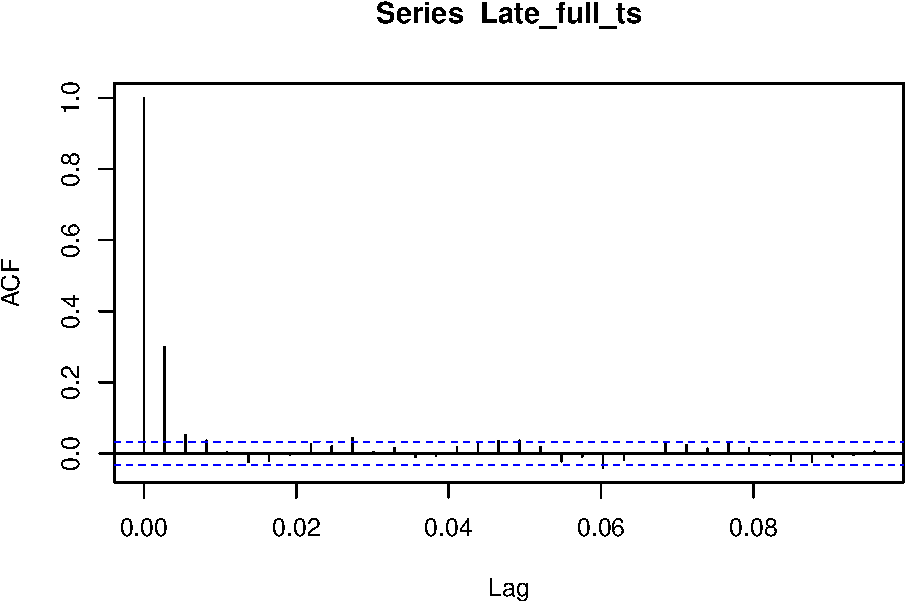
\includegraphics{Project_Template_TLK_files/figure-latex/unnamed-chunk-1-1.pdf}

\begin{Shaded}
\begin{Highlighting}[]
\FunctionTok{pacf}\NormalTok{(Late\_full\_ts) }
\end{Highlighting}
\end{Shaded}

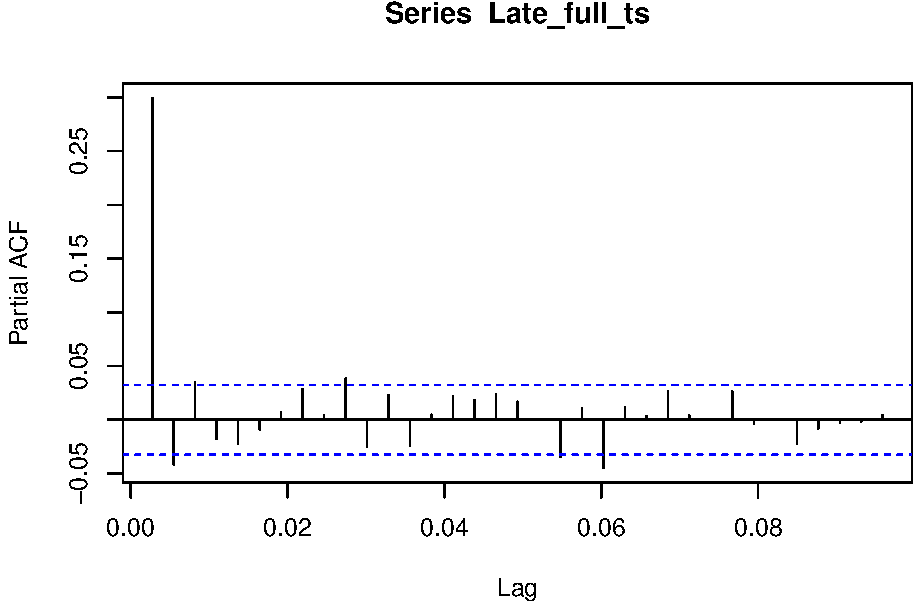
\includegraphics{Project_Template_TLK_files/figure-latex/unnamed-chunk-1-2.pdf}

\begin{Shaded}
\begin{Highlighting}[]
\FunctionTok{acf}\NormalTok{(Late\_sig\_ts)}
\end{Highlighting}
\end{Shaded}

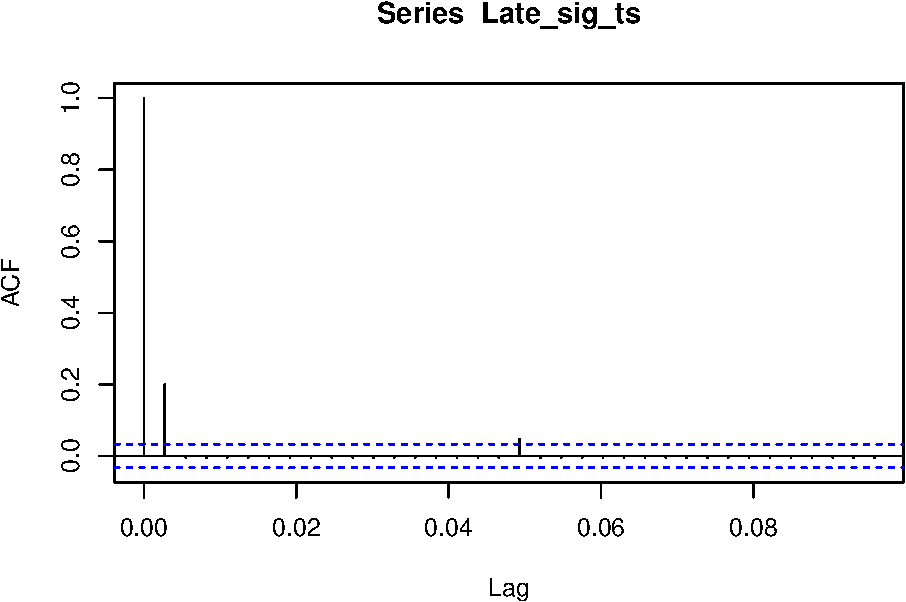
\includegraphics{Project_Template_TLK_files/figure-latex/unnamed-chunk-1-3.pdf}

\begin{Shaded}
\begin{Highlighting}[]
\FunctionTok{pacf}\NormalTok{(Late\_sig\_ts)}
\end{Highlighting}
\end{Shaded}

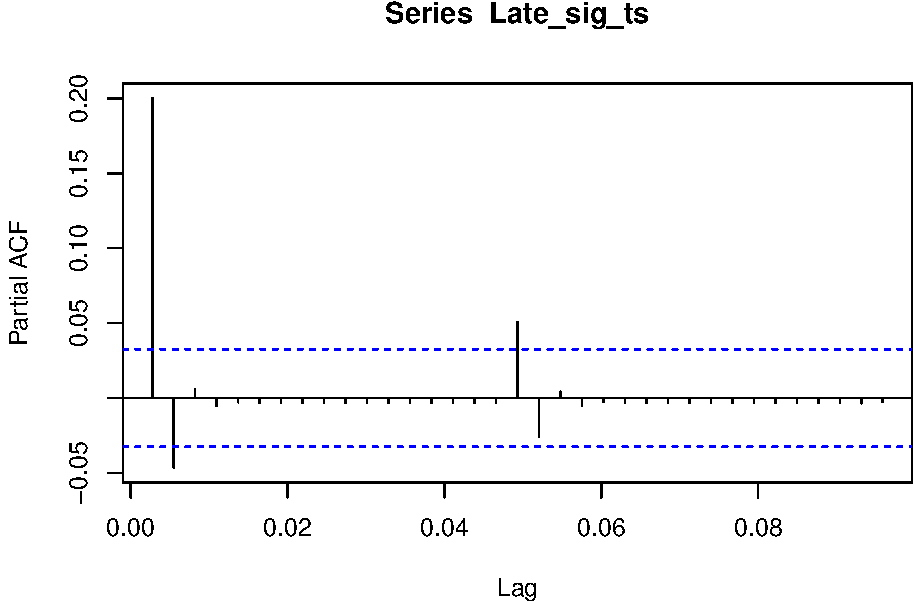
\includegraphics{Project_Template_TLK_files/figure-latex/unnamed-chunk-1-4.pdf}

\begin{Shaded}
\begin{Highlighting}[]
\FunctionTok{acf}\NormalTok{(Early\_full\_ts)}
\end{Highlighting}
\end{Shaded}

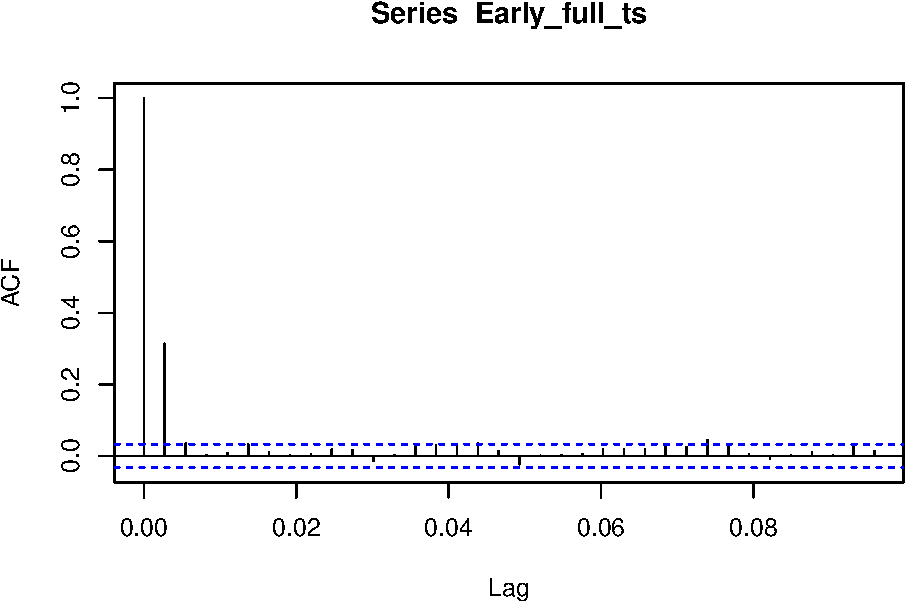
\includegraphics{Project_Template_TLK_files/figure-latex/unnamed-chunk-1-5.pdf}

\begin{Shaded}
\begin{Highlighting}[]
\FunctionTok{pacf}\NormalTok{(Early\_full\_ts)}
\end{Highlighting}
\end{Shaded}

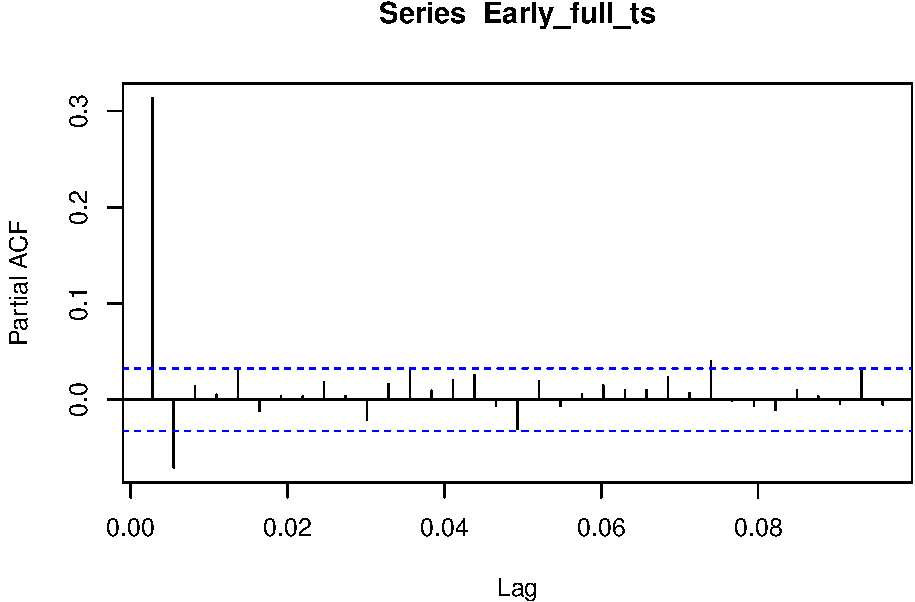
\includegraphics{Project_Template_TLK_files/figure-latex/unnamed-chunk-1-6.pdf}

\begin{Shaded}
\begin{Highlighting}[]
\FunctionTok{acf}\NormalTok{(Early\_sig\_ts)}
\end{Highlighting}
\end{Shaded}

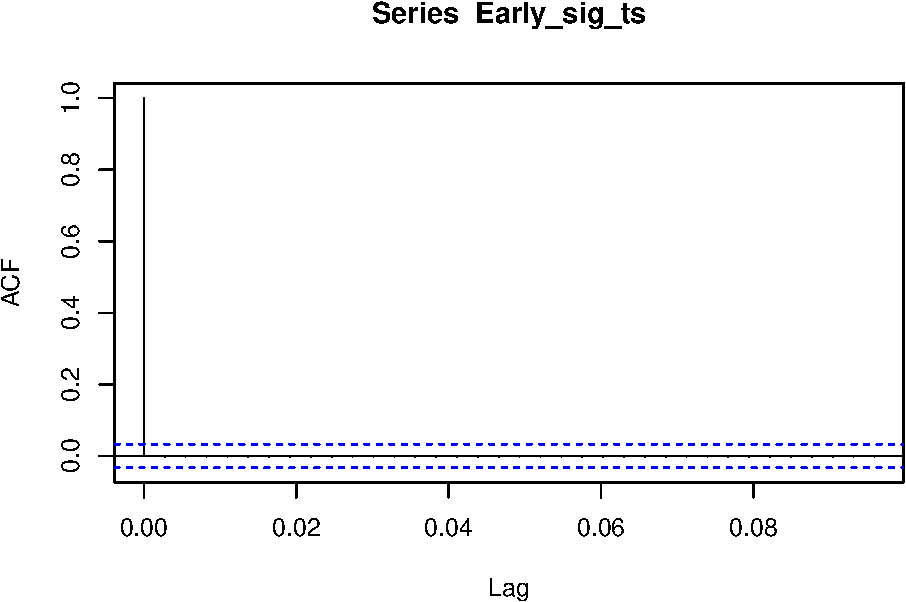
\includegraphics{Project_Template_TLK_files/figure-latex/unnamed-chunk-1-7.pdf}

\begin{Shaded}
\begin{Highlighting}[]
\FunctionTok{pacf}\NormalTok{(Early\_sig\_ts)}
\end{Highlighting}
\end{Shaded}

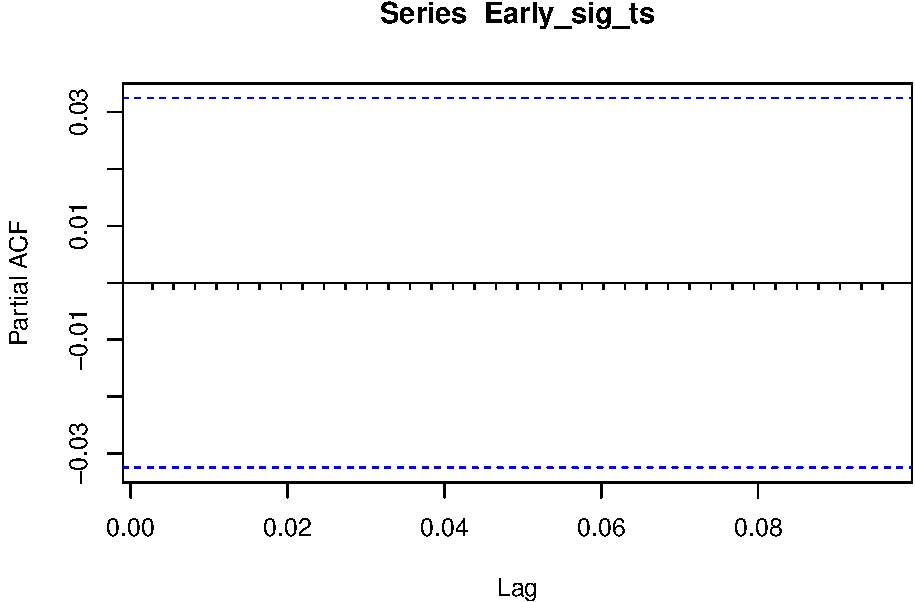
\includegraphics{Project_Template_TLK_files/figure-latex/unnamed-chunk-1-8.pdf}

\hypertarget{rationale-and-research-questions}{%
\section{Rationale and Research
Questions}\label{rationale-and-research-questions}}

Hypothesis: There is a significant increase in significant storm events
in Beaufort, NC

We will be looking at the trends of precipitation over time for
Beaufort, NC.

\newpage

\hypertarget{dataset-information}{%
\section{Dataset Information}\label{dataset-information}}

** Significant precipitation events are considered ``1 year events''
using NOAA.

\newpage

\hypertarget{exploratory-analysis}{%
\section{Exploratory Analysis}\label{exploratory-analysis}}

\newpage

\hypertarget{analysis}{%
\section{Analysis}\label{analysis}}

\begin{Shaded}
\begin{Highlighting}[]
\CommentTok{\#plot data to see possible trend}
\end{Highlighting}
\end{Shaded}

\hypertarget{question-1-is-there-is-an-increase-in-precipitation-over-time-at-beaufort-nc}{%
\subsection{Question 1: Is there is an increase in precipitation over
time at Beaufort,
NC?}\label{question-1-is-there-is-an-increase-in-precipitation-over-time-at-beaufort-nc}}

\begin{itemize}
\tightlist
\item
  We will be using a Seasonal Kendall-Mann test to determine any trends
  in precipitation data.
\item
  We will be using Seasonal Mann-Kendall test because precipitation has
  seasonal trends. We want to look at the precipitation trends without
  the variable of seasonality.
\end{itemize}

\hypertarget{question-2-is-there-an-increase-in-precipitation-by-decade}{%
\subsection{Question 2: Is there an increase in precipitation by
decade?}\label{question-2-is-there-an-increase-in-precipitation-by-decade}}

\begin{itemize}
\tightlist
\item
  We will first visually compare the number of significant precipitation
  events for each decade, then run a t-test to determine if there is a
  significant difference in number of significant precipitation events
  comparing decades.
\end{itemize}

\newpage

\hypertarget{summary-and-conclusions}{%
\section{Summary and Conclusions}\label{summary-and-conclusions}}

\newpage

\hypertarget{references}{%
\section{References}\label{references}}

\textless add references here if relevant, otherwise delete this
section\textgreater{}

\end{document}
